\title{Umělá inteligence}

\section{Umělá inteligence(UI) - Definice, úzká UI obecná UI, superinteligence, strojové učení}
Umělá intelgince je výpočetní systém vykonávající činnost, kterou si spojujeme s lidskou inteligencí\\
Další definice: 
\begin{itemize}
    \item počítačové systémy, které jsou schopné plnit úkoly, které obvykle vyžadují lidskou inteligenci, jako je rozhodování, detekce objektů, řešení složitých problémů
    \item vědní disciplína, zabývající se teoríí systémů zpracovávajících data a schopných se víceméně samostatně rozhodovat
    \item schopnosti počítače/algoritmu napodobovat/realizovat některé funkce lidského mozku
\end{itemize}
\subsection*{Úzká umělá inteligence}
stupeň UI zahrnující stroje, které mohou provádět pouze úzce definovaou sadu konkrétních úkolů\\
jediná forma, které lidstvo doposud dosáhlo\\
aplikace na rutinních pracích - rozpoznávání řeči, obrazu, počítačové vidění, inteligentní budovy, hra šachů, návrh nákupu, počasí\\
UI je vznešený název pro sofistikované SW řešení, vkládáme důvěru do autora, že nic neopomenul\\
\begin{figure}[H]
    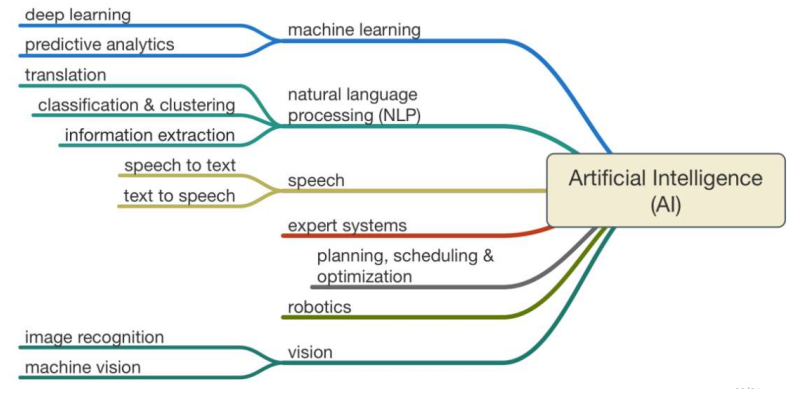
\includegraphics[scale = 1]{images/uzkeAI.png}
\end{figure}
\subsection*{Obecná UI}
Umělá inteligence na úrovni člověka\\
umí se rozhodovat, komunikovat, samostatně se učit\\
zatím není vyvinuta\\
Tuninguv test - nemožnost rozeznat člověka od stroje\\

\subsection*{Superinteligence}
má vyšší inteligenci než člověk\\
uvědomuje si, že ji ovládají a omezují intelektuálně podřadní lidé\\



\subsection*{Strojové učení(machine learning)}
\begin{itemize}
    \item zaměření na to, aby se stroje rozohodovaly na základě dat
    \item techniky strojového učení:
    \item \begin{itemize}
        \item učení s učitelem
        \item učení bez učitele
        \item zpětnovazební učení, posílené učení
    \end{itemize}
\end{itemize}
Učení s učitelem:
\label{typ_uceni}
\begin{figure}[H]
    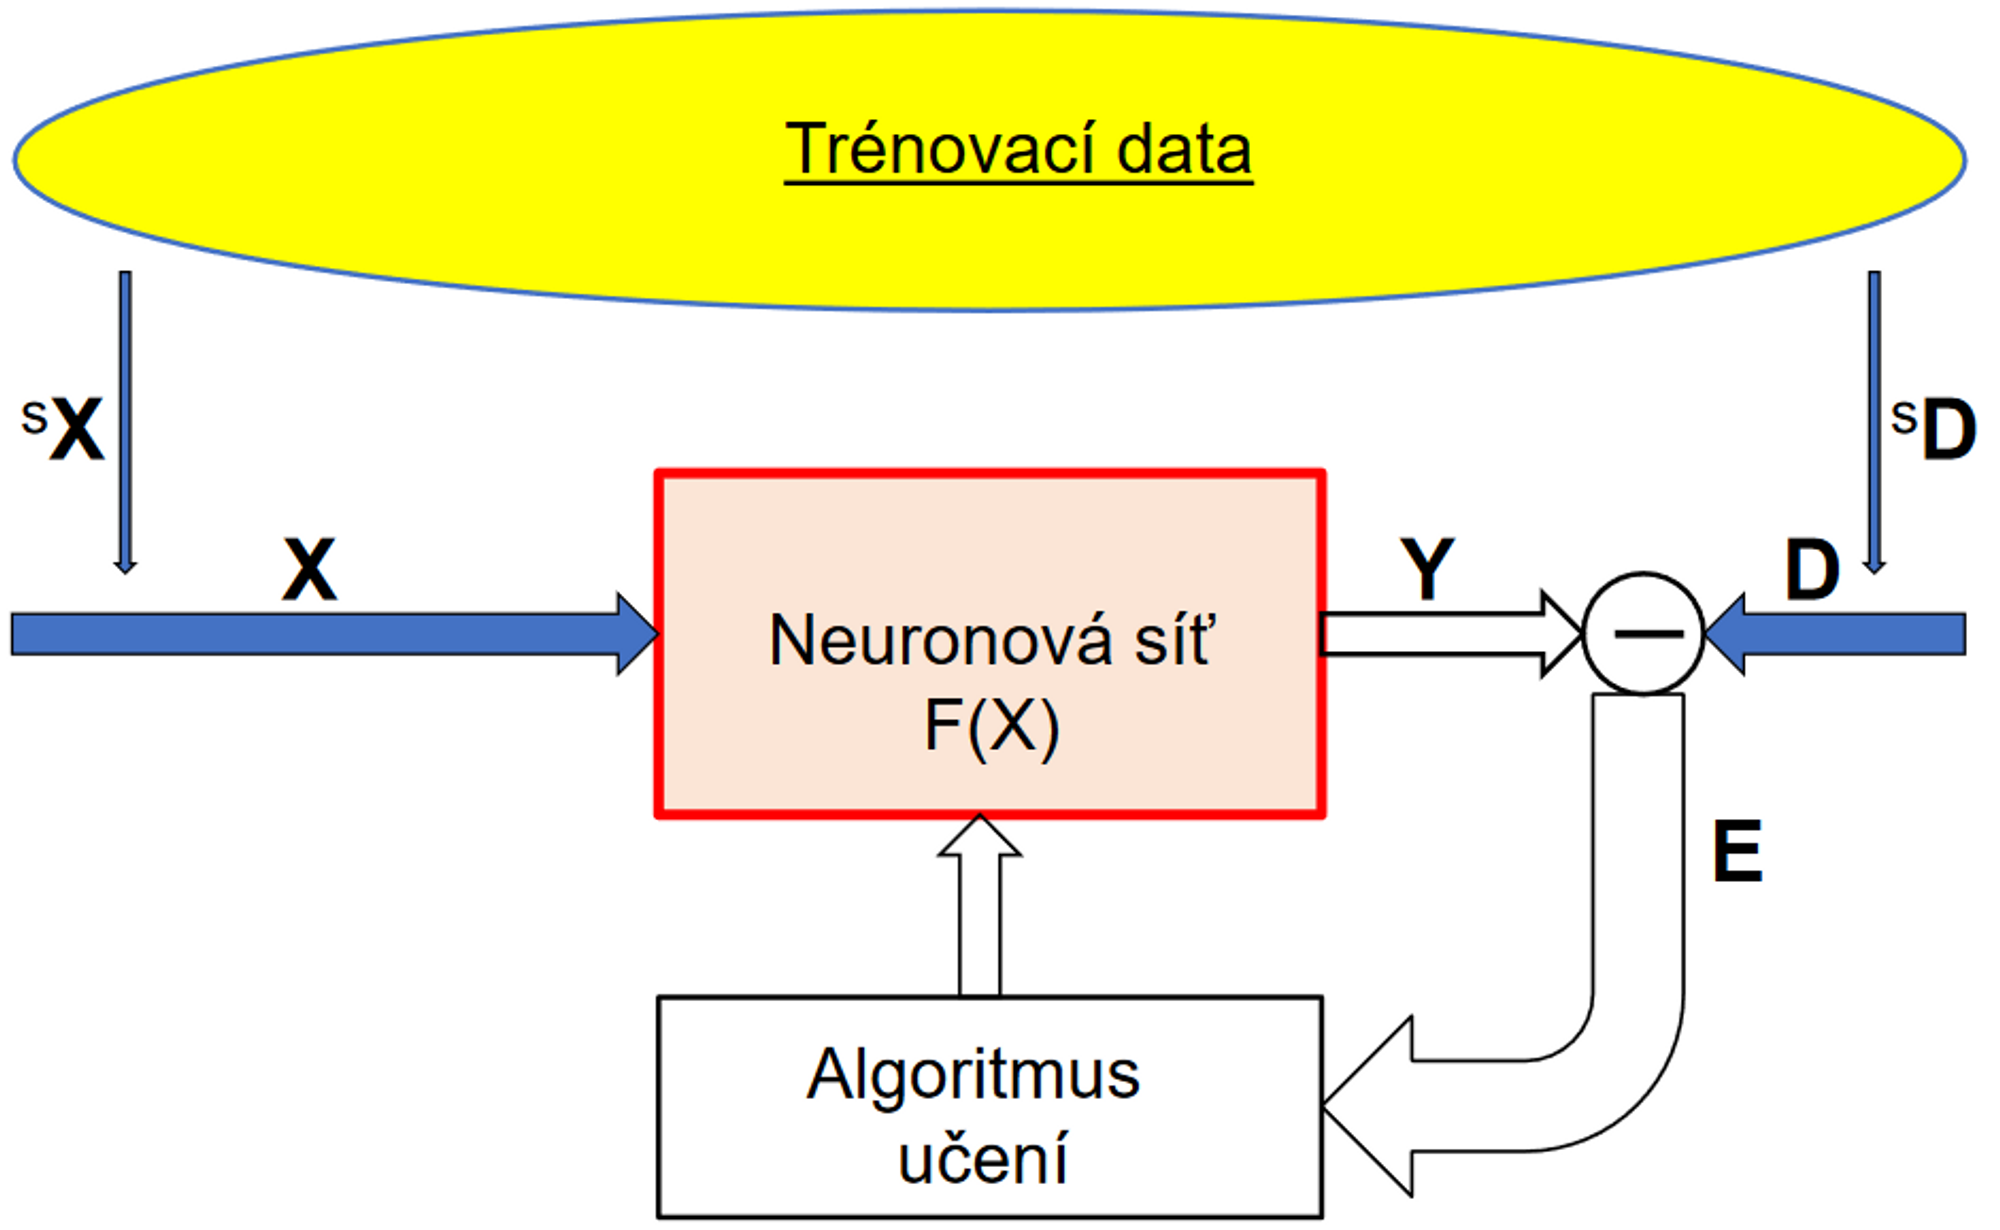
\includegraphics[scale = 0.3]{images/sUcitelem.png}
\end{figure}
Data jsou rozdělena na trénovací, validační a testovací\\
Učení probíhá tak, že systému předkládáme trénovací vzory a zároveň požadované výstupy, na základě kterých se mění váhy.\\
\newpage
Učení bez učitele:
\begin{figure}[H]
    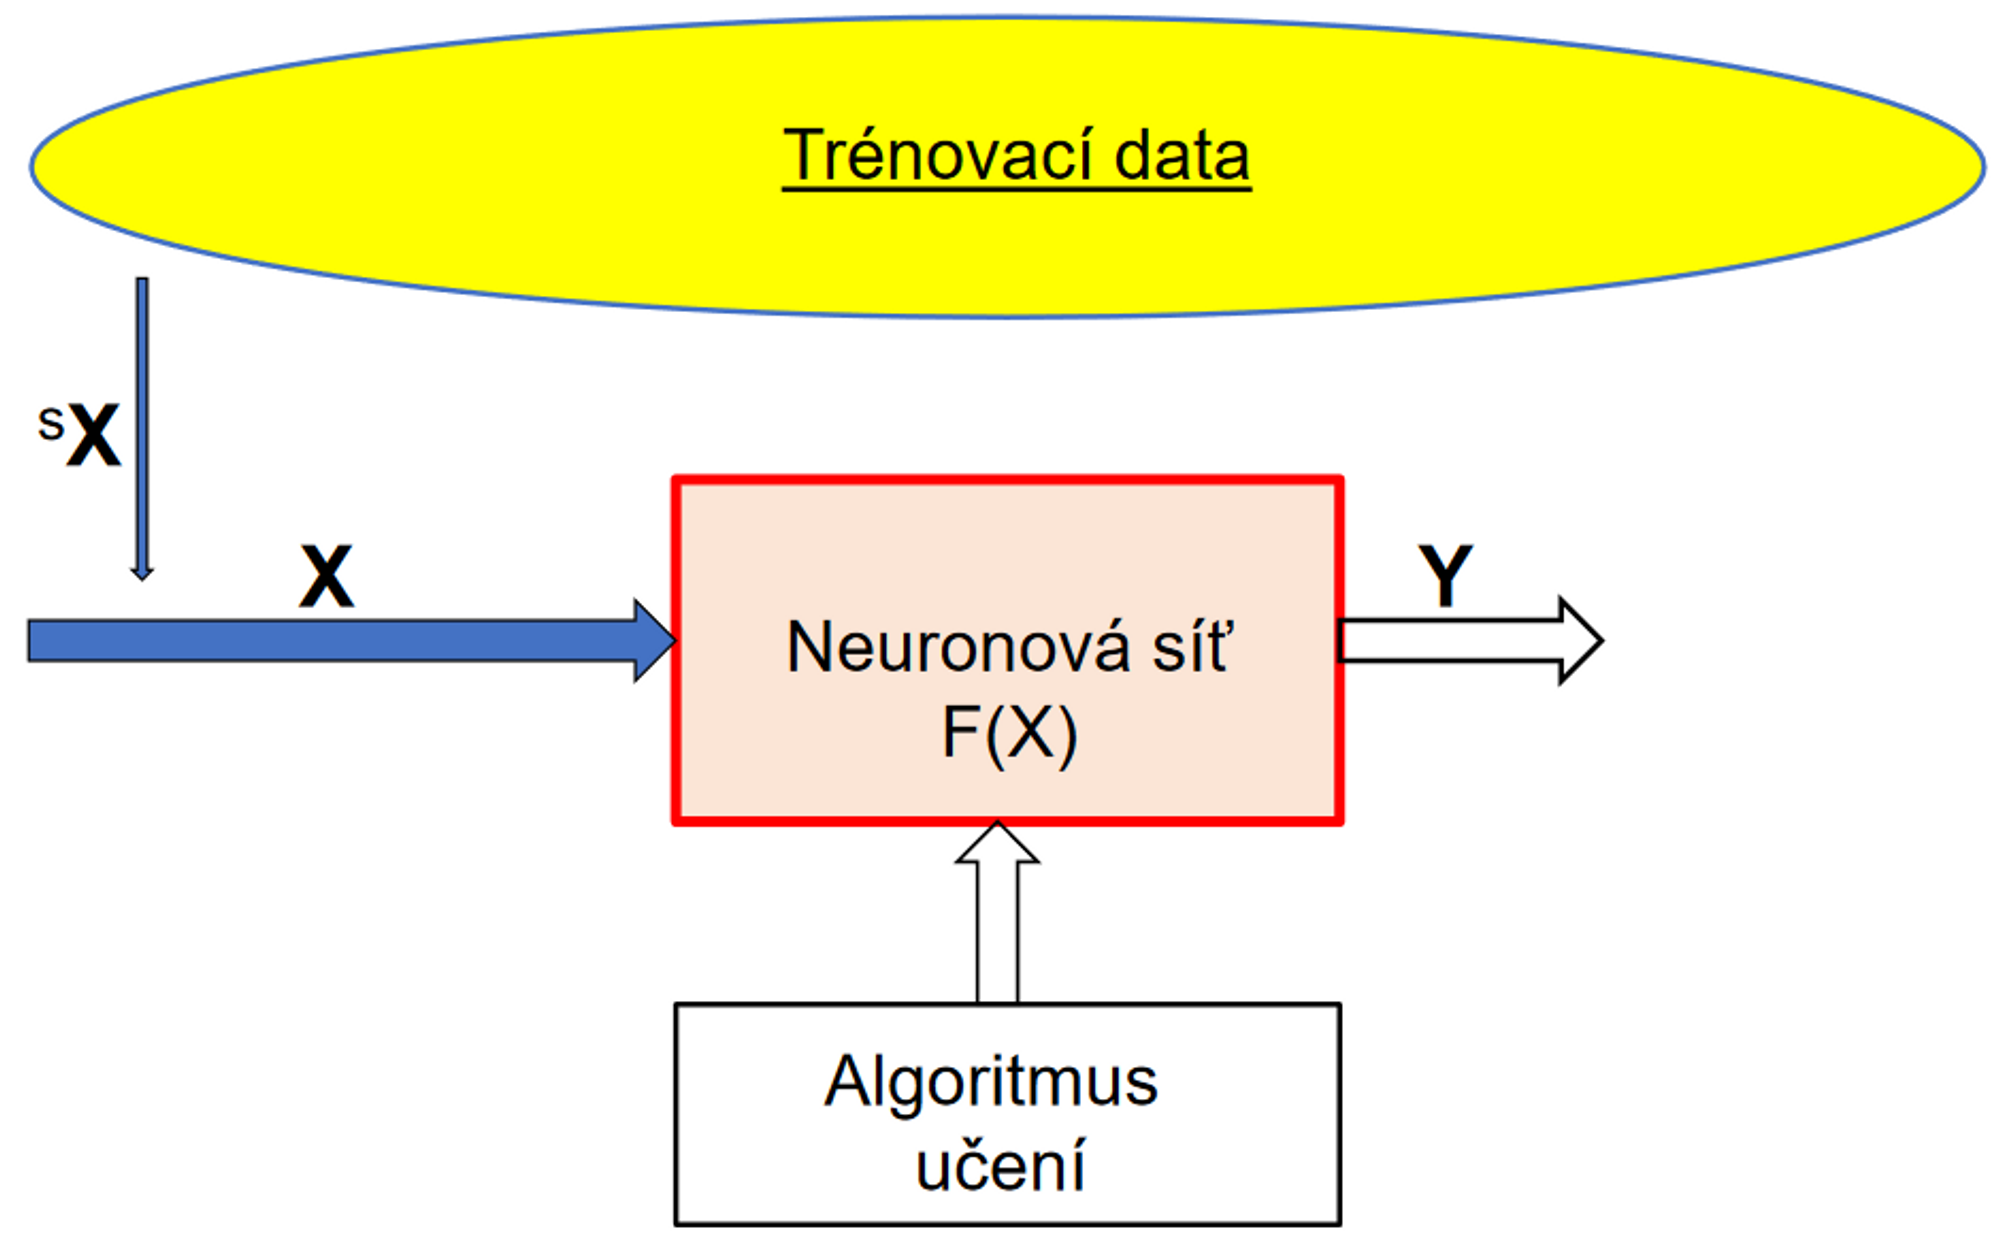
\includegraphics[scale = 0.4]{images/bezUcitele.png}
\end{figure}
Data jsou pouze jednoho typu a to trénovací\\
Učení probíhá tak, že jsou systému předloženy sady vstupů(bez správných výsledků, protože je neznáme) a na základě vstupů se mění váhy.\\

Existuje i kombinace obou přístupů, nazývá se expectation maximization algoritmus.

\subsection*{Základní druhy úloh}
\begin{itemize}
    \item Klasifikace vstupních dat do tříd
    \item Odhadování výstupní hodnoty podle vstupu
    \item Zařazování objektů do skupin podle podobných vlastností - učení bez učitele
\end{itemize}

\section{Umělé neuronové sítě - paradigmata, perceptron, algoritmus Backpropagation, Kohonenova samoorganizační mapa, konvoluční neuronová síť}
\subsection*{Paradigmata}
použité modely neuronů\\
topologie\\
způsob učení\\
způsob vybavování\\

\subsubsection*{Neuron}
\begin{figure}[H]
    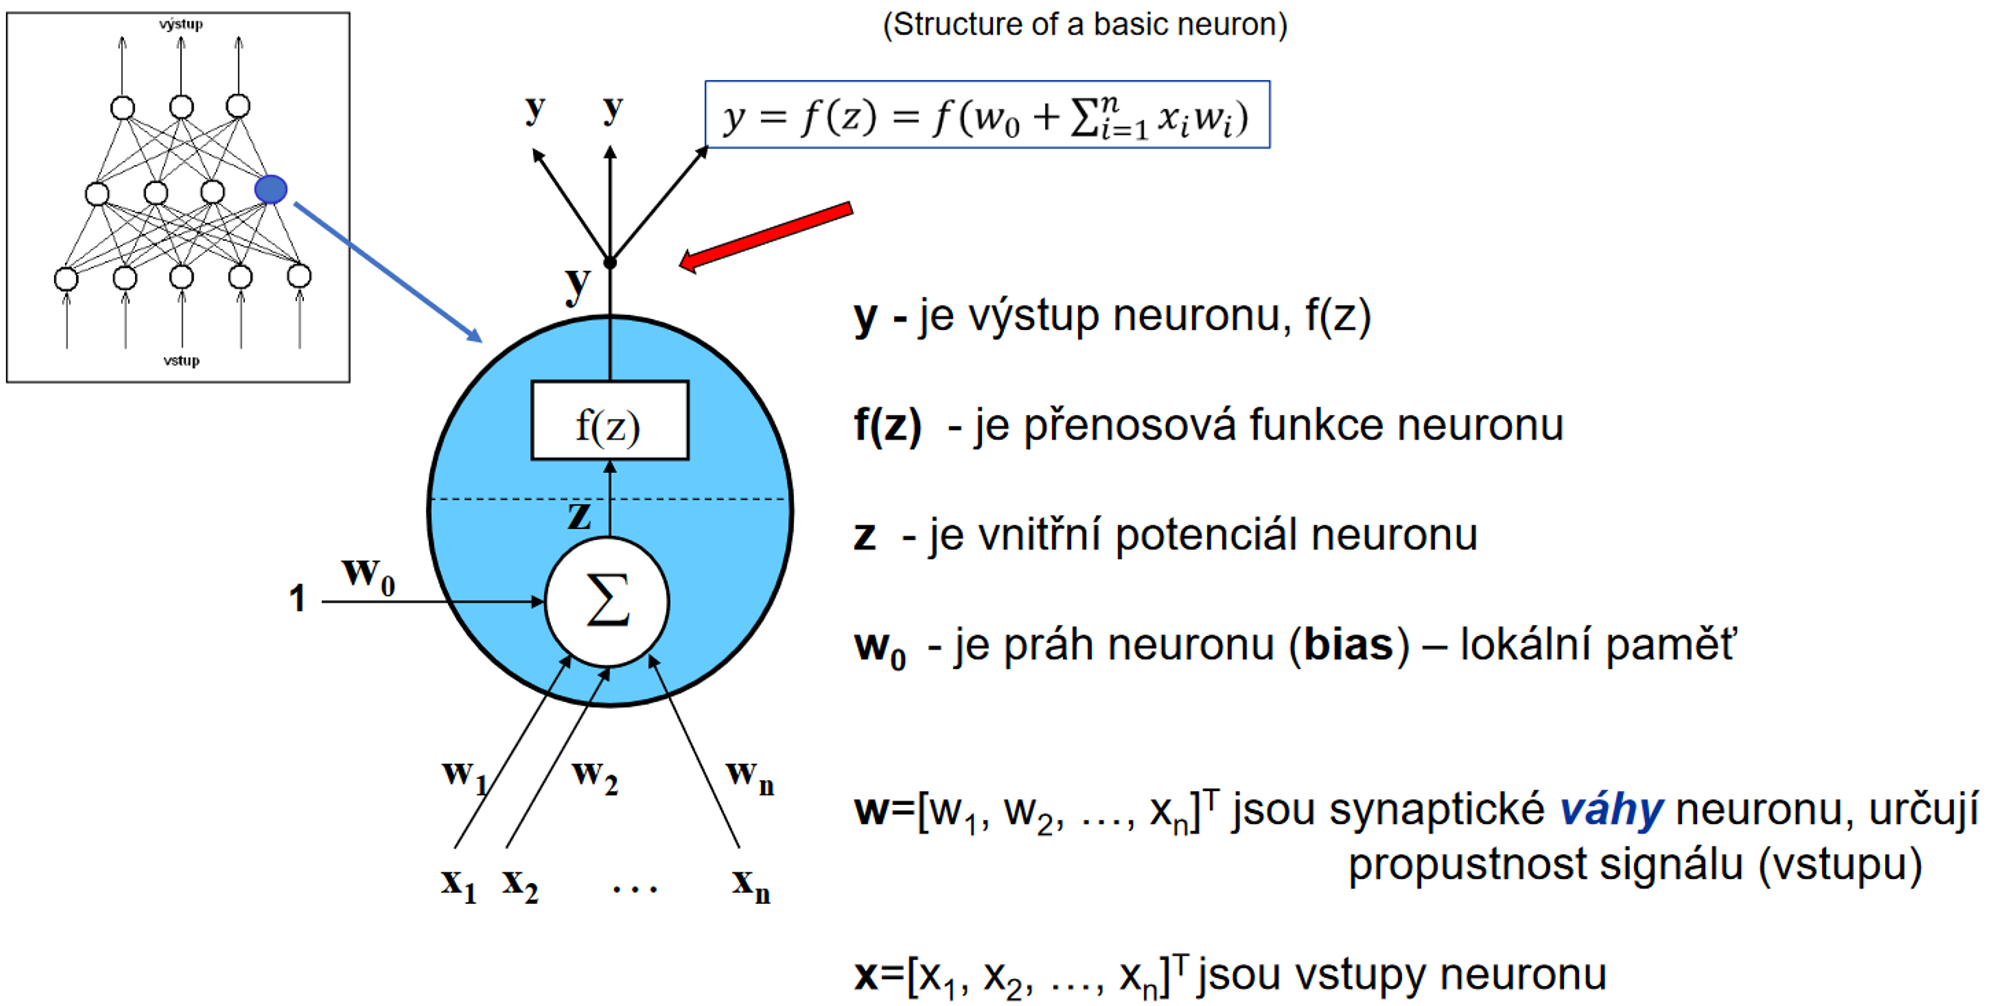
\includegraphics[scale = 0.5]{images/neuron.png}
\end{figure}
vnitřní potenciál neuronu je lineární, nebo radiální
\begin{itemize}
    \item lineární: $z = w_0 + \sum^n_{i=1}x_iw_i$
    \item radiální: $z = w_0 + \sqrt{\sum^n_{i=1}(x_i-w_i)^2}$
\end{itemize}

\subsubsection*{Topologie}
Orientovaný graf
\begin{itemize}
    \item neurony tvoří uzly grafu
    \item hrany grafu se nazývají spoje 
    \item každý spoj má váhu
    \item každý neuron má libovolný počet vstupů a výstupů(stejných)
    \item každý neuron má bias, vnitřní potencíál a přenosovou funkci
\end{itemize}
struktura je Přímovazební nebo zpětnovazební:
\begin{figure}[H]
    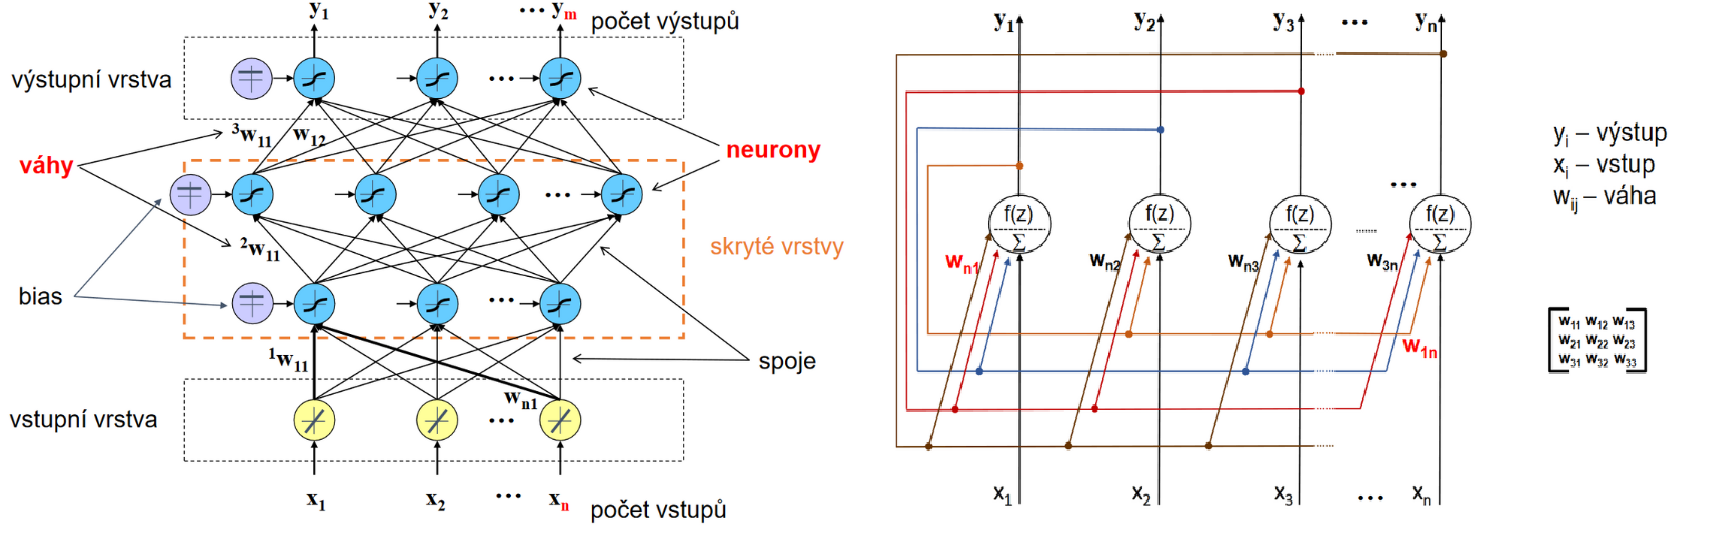
\includegraphics[scale = 0.5]{images/struktury.png}
\end{figure}

\subsubsection*{Učení popsáno v předchozí otázce viz \ref{typ_uceni}}

\subsubsection*{Vybavování}
aktivní režim\\
vlastní výpočet funkce naučené neuronové sítě na daný vstup\\
jsou dva typy:
\begin{itemize}
    \item jednorázový - přímovazební, odezva probíhá v jedné iteraci
    \item iterační proces - zpětnovazební, odezva probíhá iterativně
\end{itemize}

\subsubsection*{Aplikace}
regrese - predikce spojité proměnné na základě vstupu\\
klasifikace - zařazení do tříd(detekce spamu, jestli poslat pacienta na dané vyšetření)\\
časové řady - jak regrese tak klasifikace\\
shluková analýza - učení 

\subsection*{Perceptron}
Charakteristika:
\begin{itemize}
    \item neuron - nespojitá přenosová funkce
    \item topologie - jednovrstvá přímovazební
    \item učení - iterativní, s učitelem
    \item tréninková množina - \textbf{lineárně separabilní}
    \item vybavování - jednorázový proces
    \item aplikace - lineárně separabilní klasifikátor
\end{itemize}
\subsubsection*{Neuron}
\begin{figure}[H]
    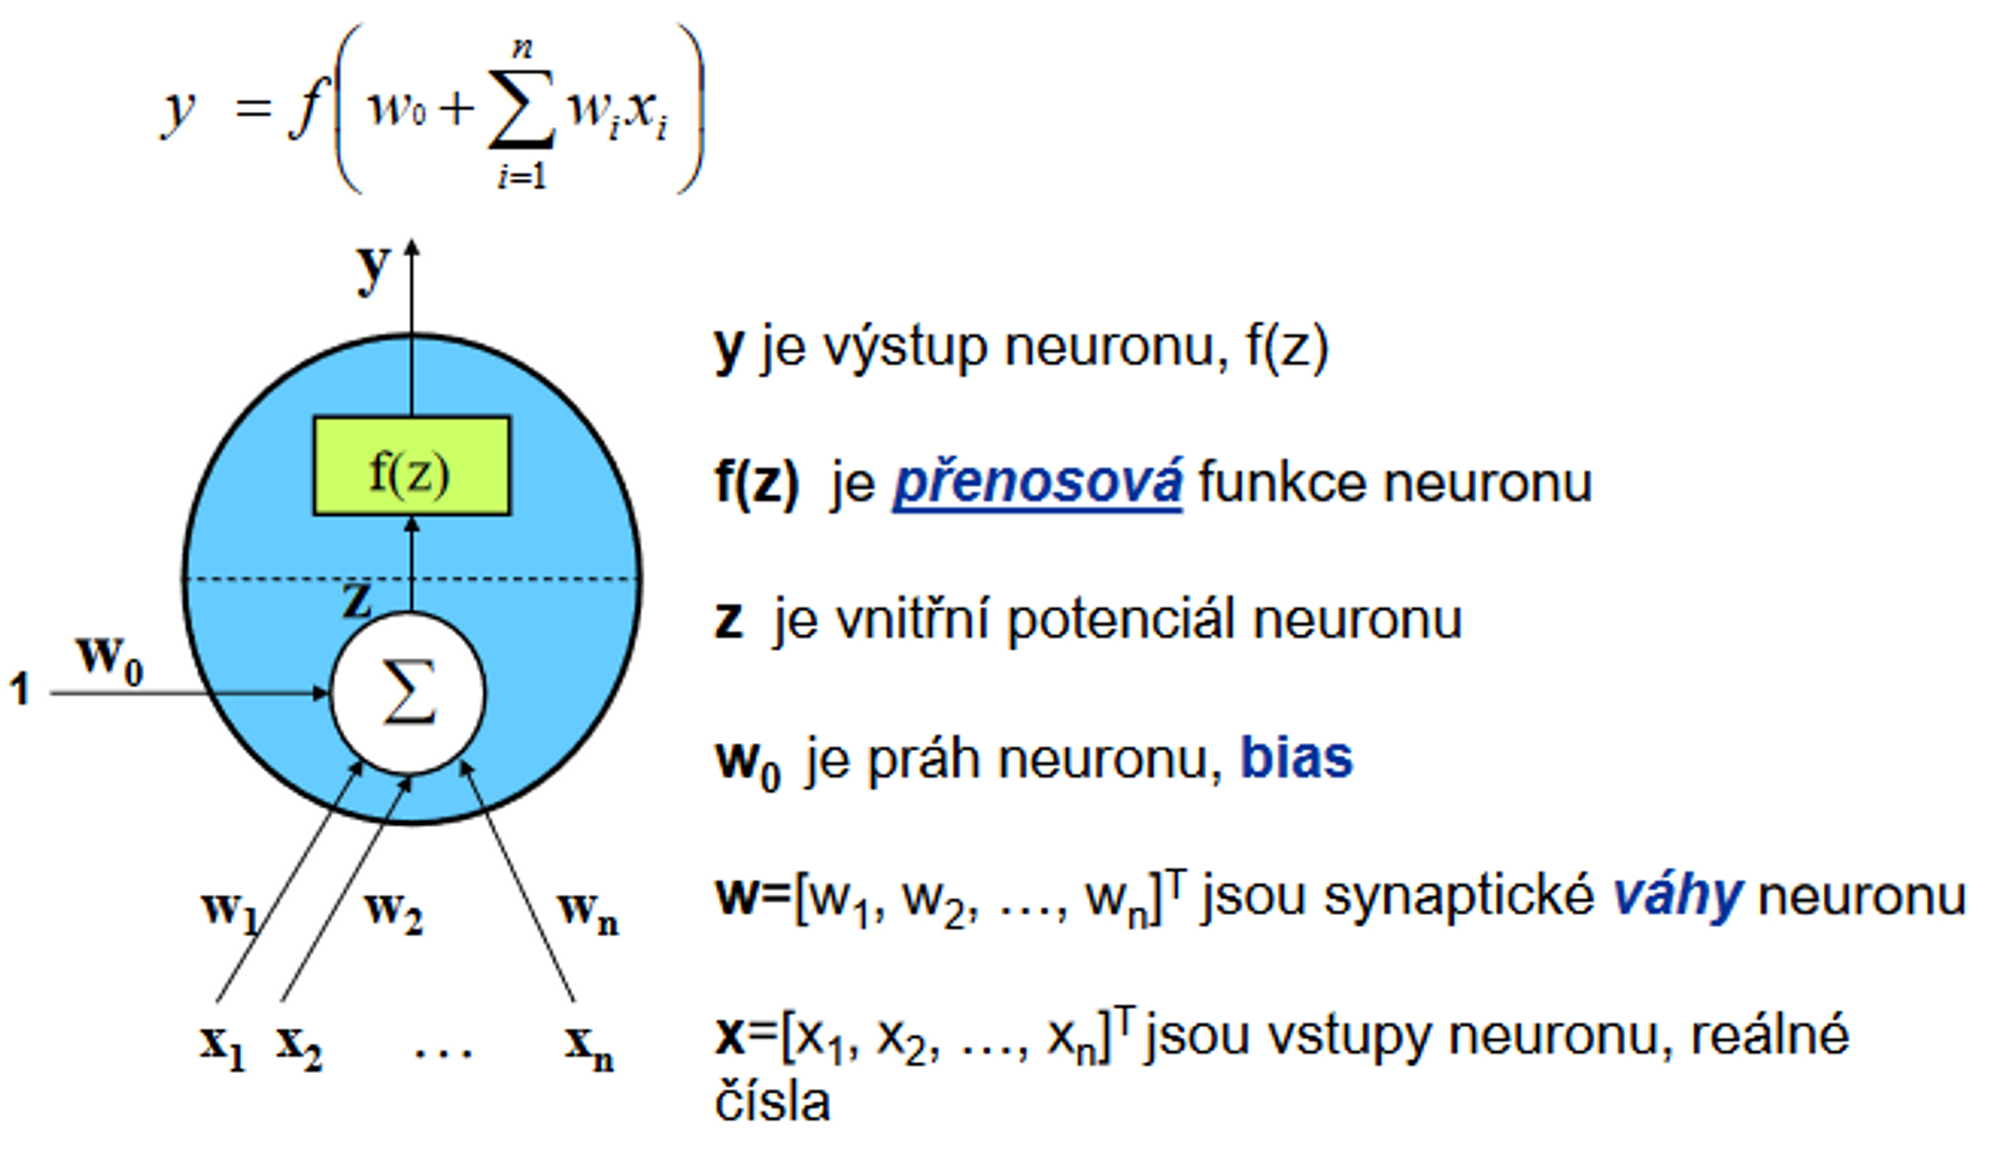
\includegraphics[scale = 0.3]{images/perceptron_neuron.png}
\end{figure}
\newpage
Přenosová funkce bez prahu:
\begin{figure}[H]
    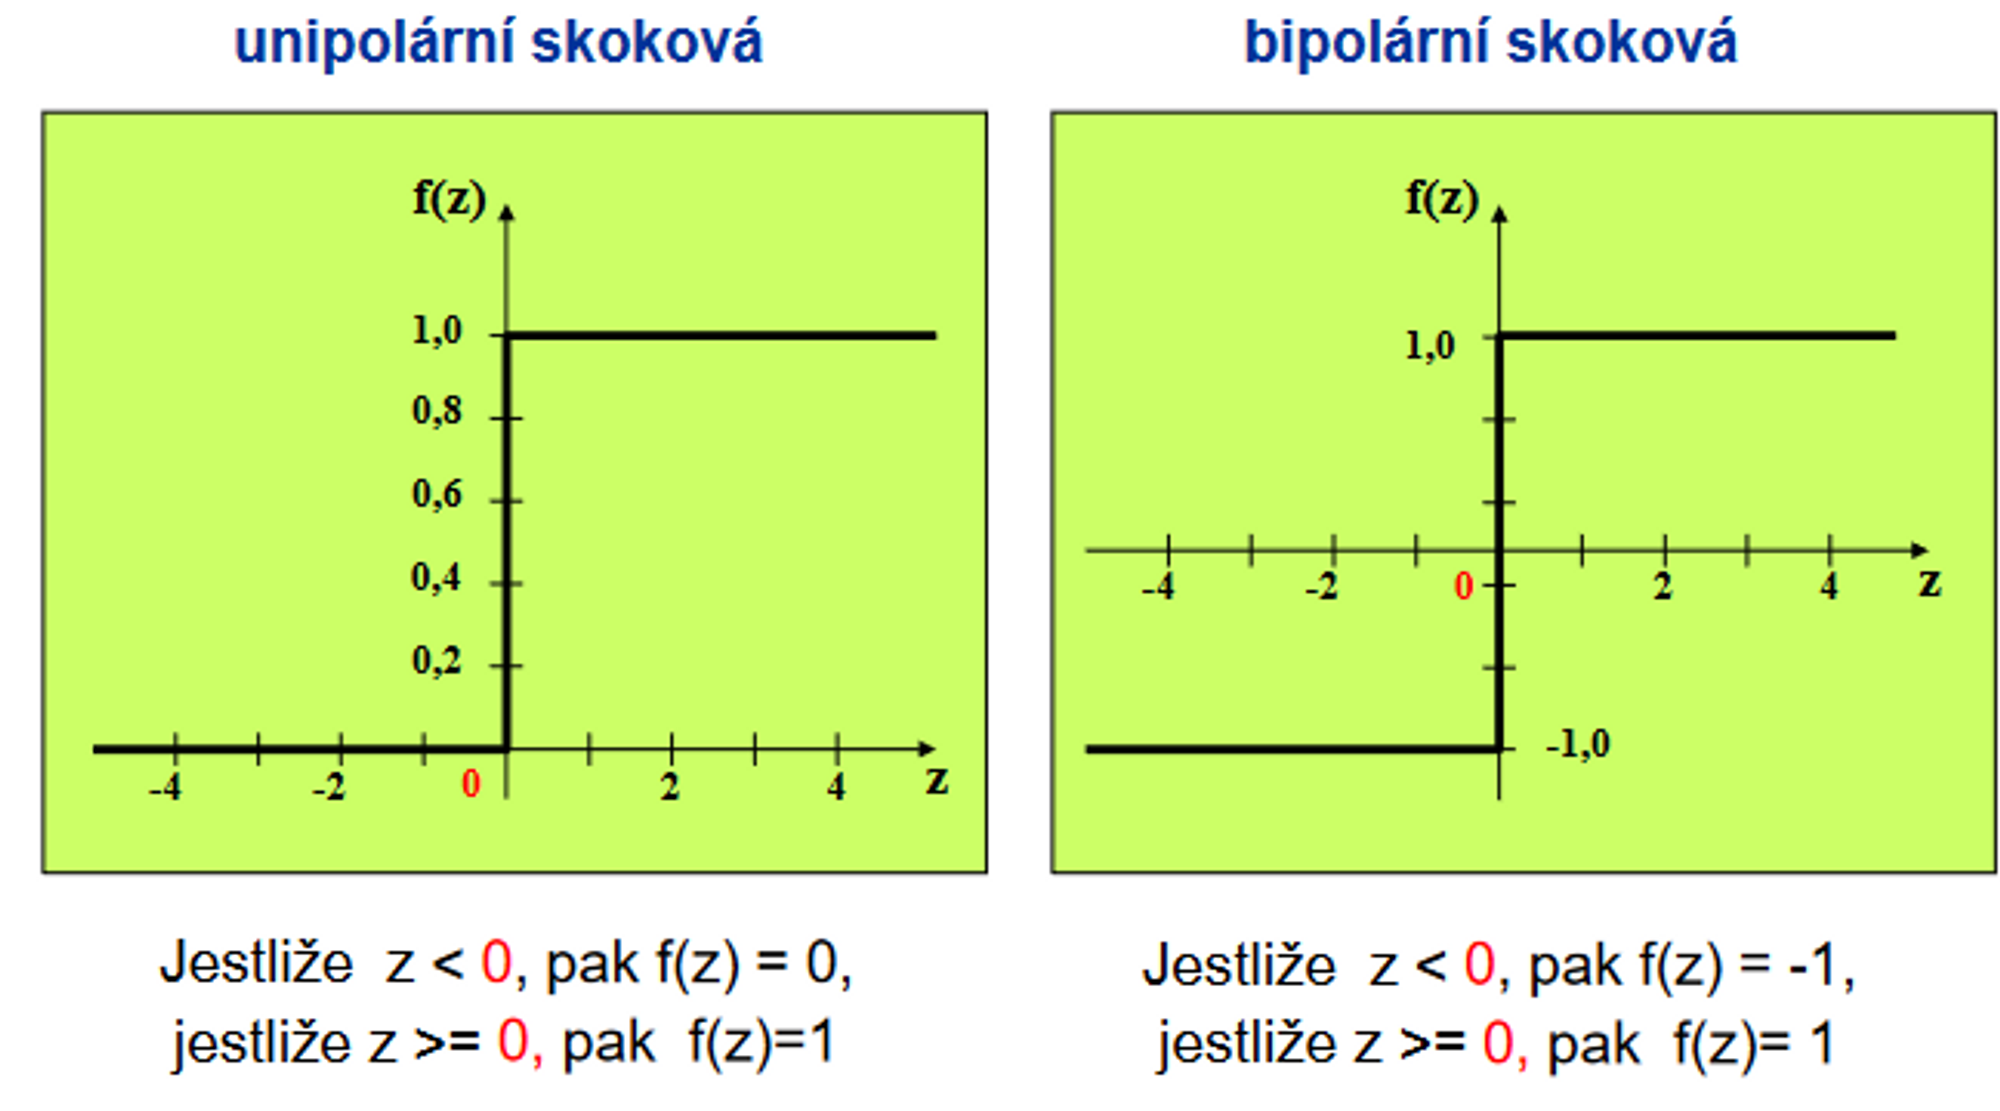
\includegraphics[scale = 0.3]{images/perceptron_prenos.png}
\end{figure}
Přenosová funkce s prahem
\begin{figure}[H]
    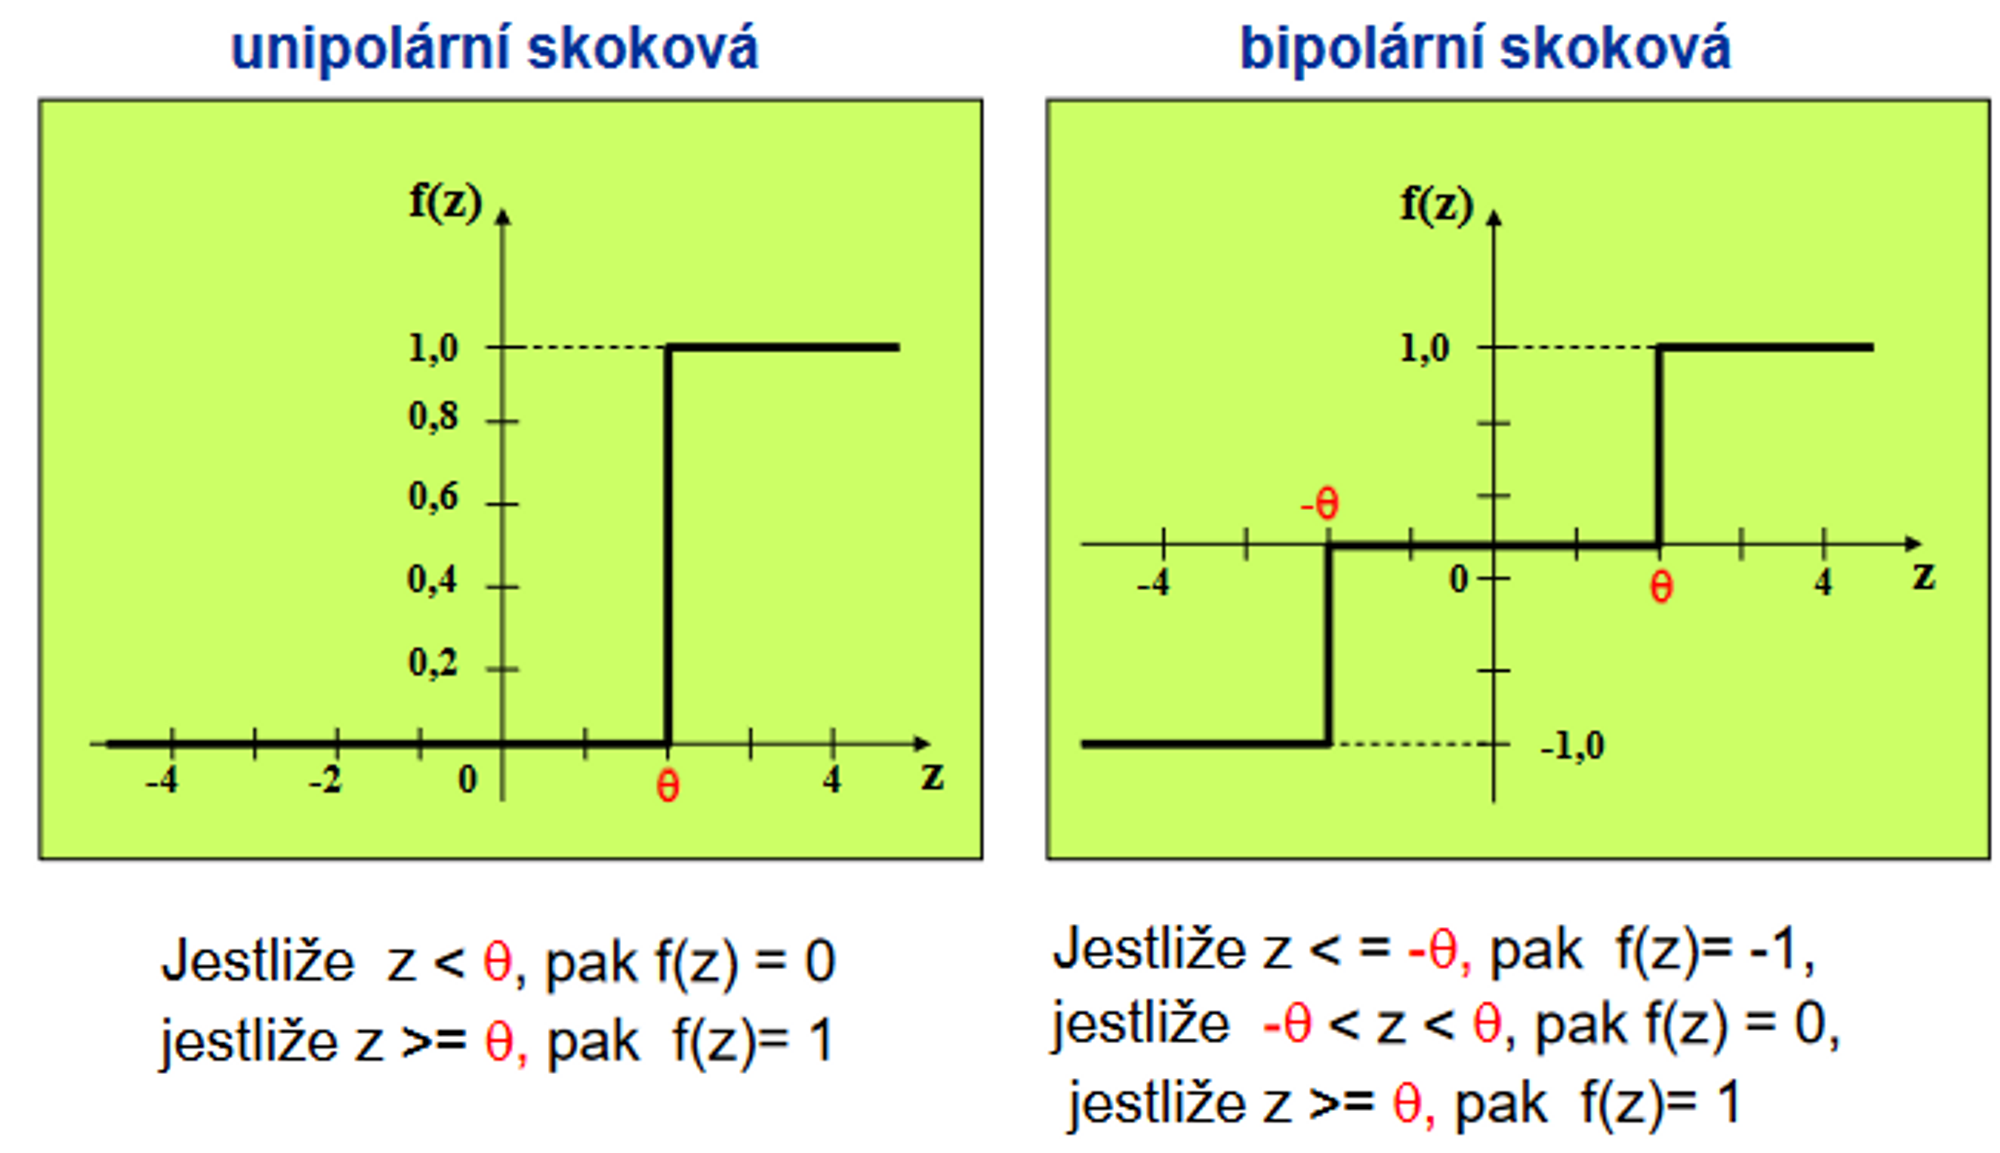
\includegraphics[scale = 0.3]{images/perceptron_prenos_s_prahem.png}
\end{figure}

\subsubsection*{Topologie}
jeden nebo více perceptronů
\newpage
\subsubsection*{Učení}
když je v n-rozměrném rostoru lineárně separabilní třída objektů, v konečném počtu kroků učení lze najít vektor vah perceptronu, který je oddělí\\
Kroky učení:
\begin{enumerate}
    \item Start, inicializace(nastavení vah a určení přenosové funkce)
    \item předložení tréninkového vzoru
    \item výpočet výstupu sítě
    \item učení - adaptace vah
    \item test na shodu
    \item test na ukončení - jestli jsou všechny klasifikace správně
\end{enumerate}
Nastavení vah je na malá náhodná čísla\\
Adaptace vah probíhá třemi různými způsoby:\\
A):
\begin{figure}[H]
    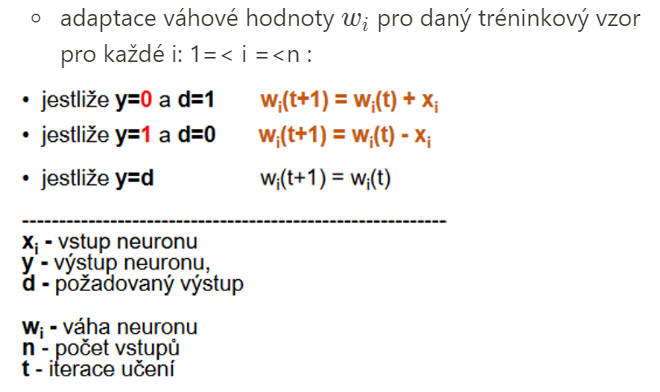
\includegraphics[scale = 1]{images/perceptron_vahy1.png}
\end{figure}
\newpage
B):
\begin{figure}[H]
    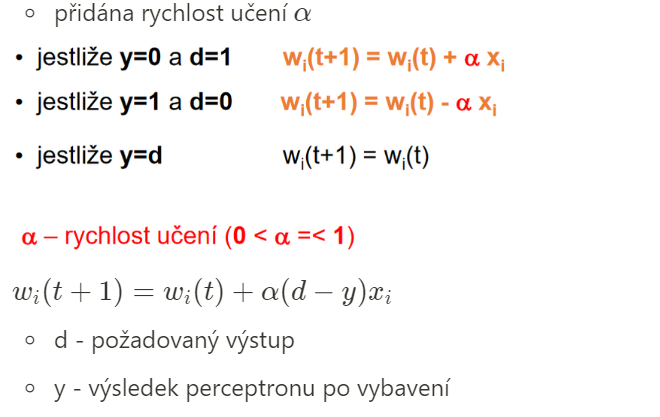
\includegraphics[scale = 1]{images/perceptron_vahy2.png}
\end{figure}
C):
\begin{figure}[H]
    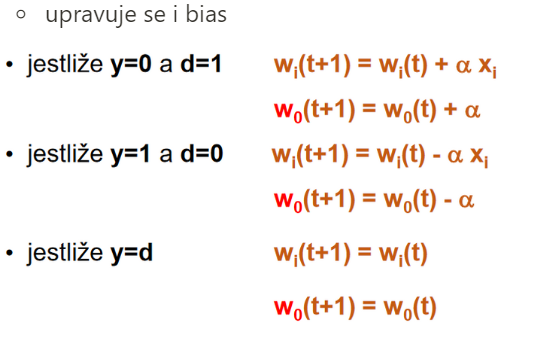
\includegraphics[scale = 1]{images/perceptron_vahy3.png}
\end{figure}

\subsubsection*{vybavování}
Výstup:
\begin{itemize}
    \item 0/1
    \item -1/1
    \item -1/0/1
\end{itemize}
\subsubsection*{Kritika perceptronu}
schopný řešit jen problémy, které jsou linárně separabilní\\
nelze realizovatfunkci XOR

\subsection*{Algoritmus Backpropagation}
Charakteristika
\begin{itemize}
    \item neuron - spojitá přenosová funkce
    \item topologie - vícevrstvá, přímovazební
    \item učení - s učitelem, iterační gradientní proces nastavení vah, algoritmus se zpětným šířením chyby
    \item vybavování - jednorázový proces
    \item aplikace - modelování nelineárních funkcí, klasifikace
\end{itemize}

\subsubsection*{Neuron}
ve vstupní vrstvě distribuce signálu, přenosová funkce lineární(nemusí mět strmost 1)\\
ostatní vrstvy přenosová funkce sigmoida(výstup 0/1), tangenta hyperbolická(-1/1)

\subsubsection*{Topologie}
minimálně 3 vrsty neuronů\\
vstupní vrstva - distrubuce signálu\\
prostřední vrstvy(skryté) - úplné propojení neuronů\\
\begin{figure}[H]
    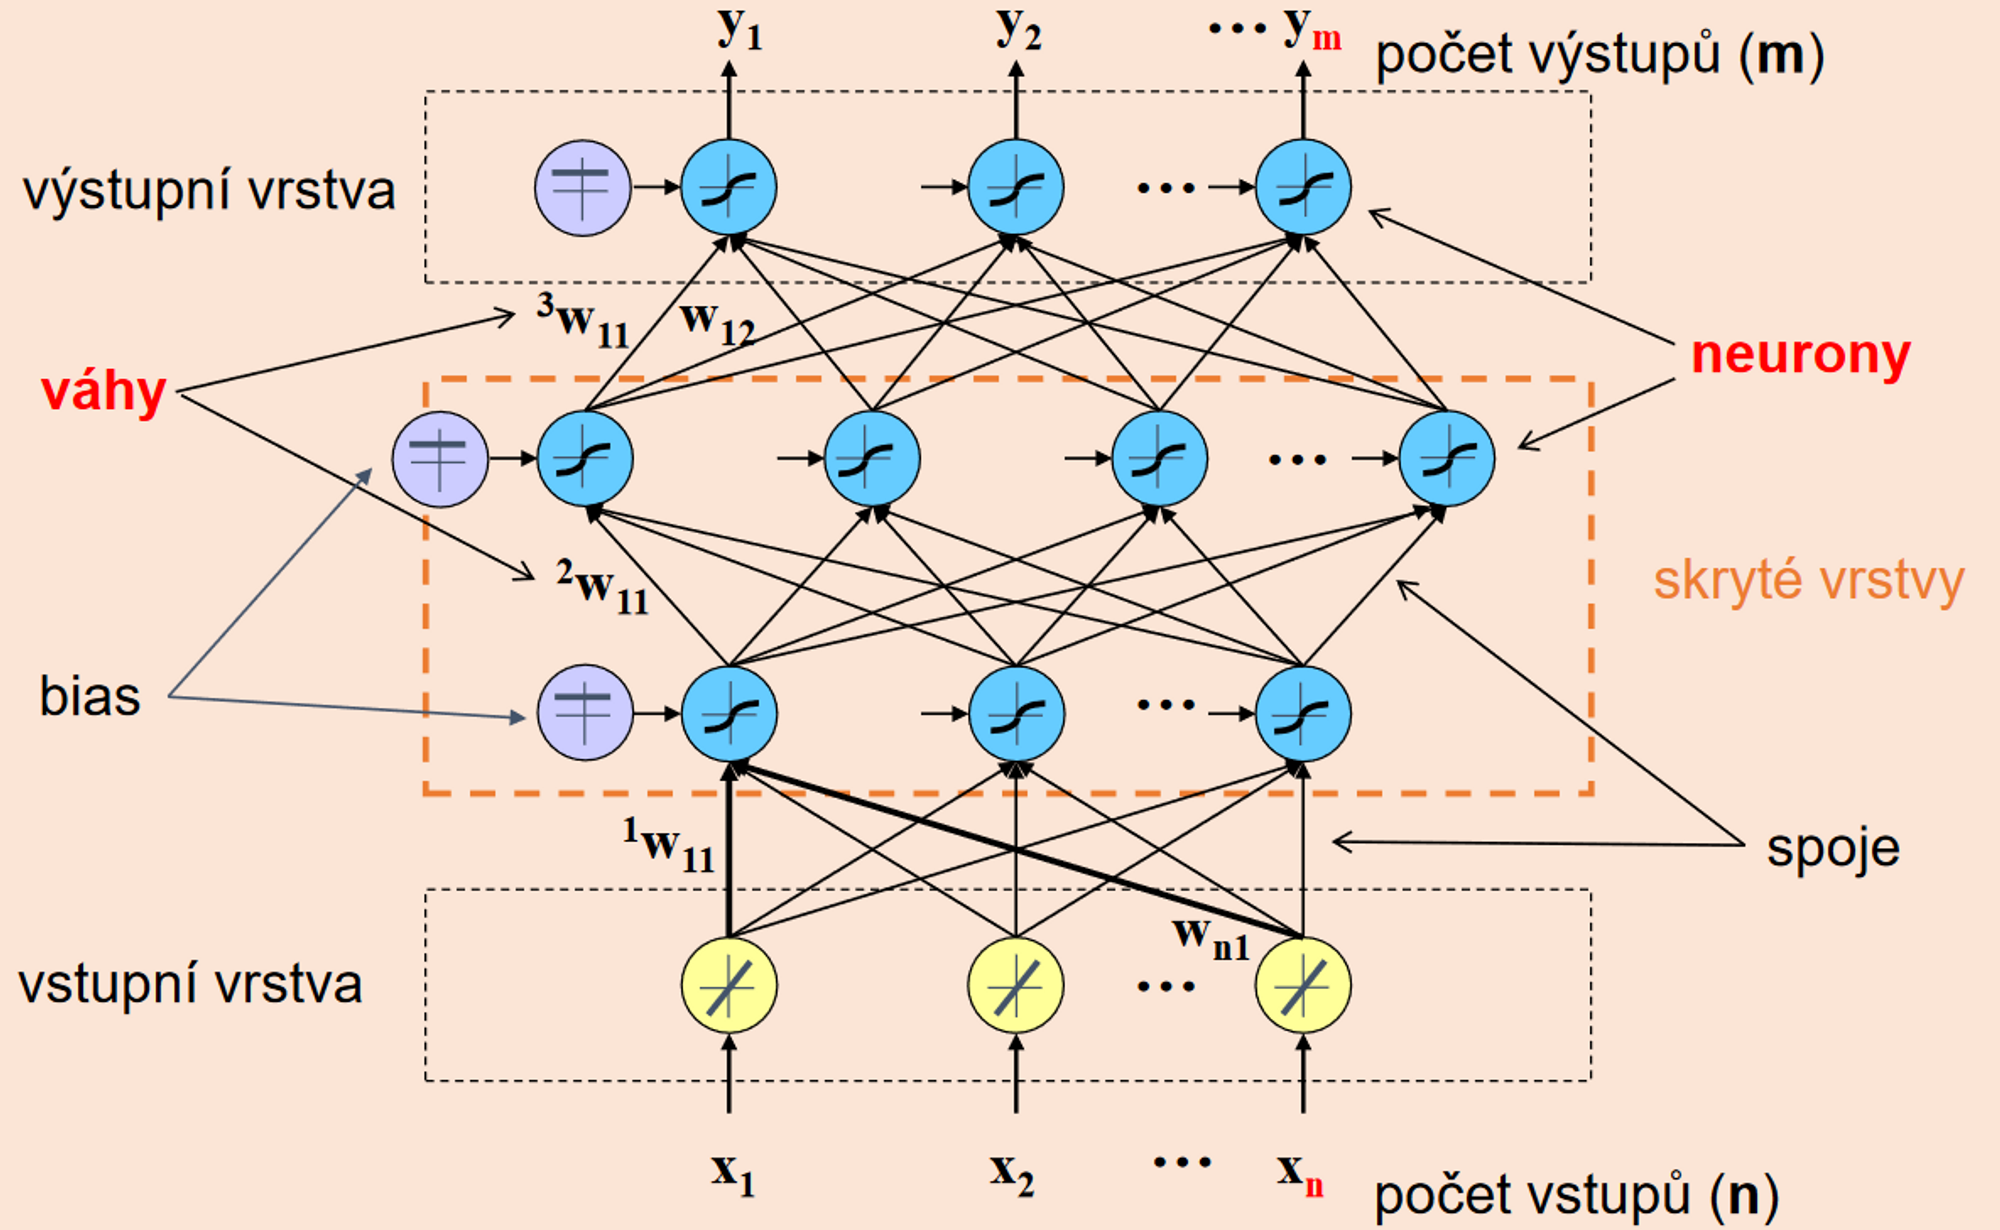
\includegraphics[scale = 0.3]{images/backPropag_topologie.png}
\end{figure}

\subsubsection*{Učení}
učení s učitelem\\
pracuje se s chybou sítě \textit{E}, což je rozdíl mezi skutečnými a požadovanými hodnotami\\
Kroky učení:
\begin{figure}[H]
    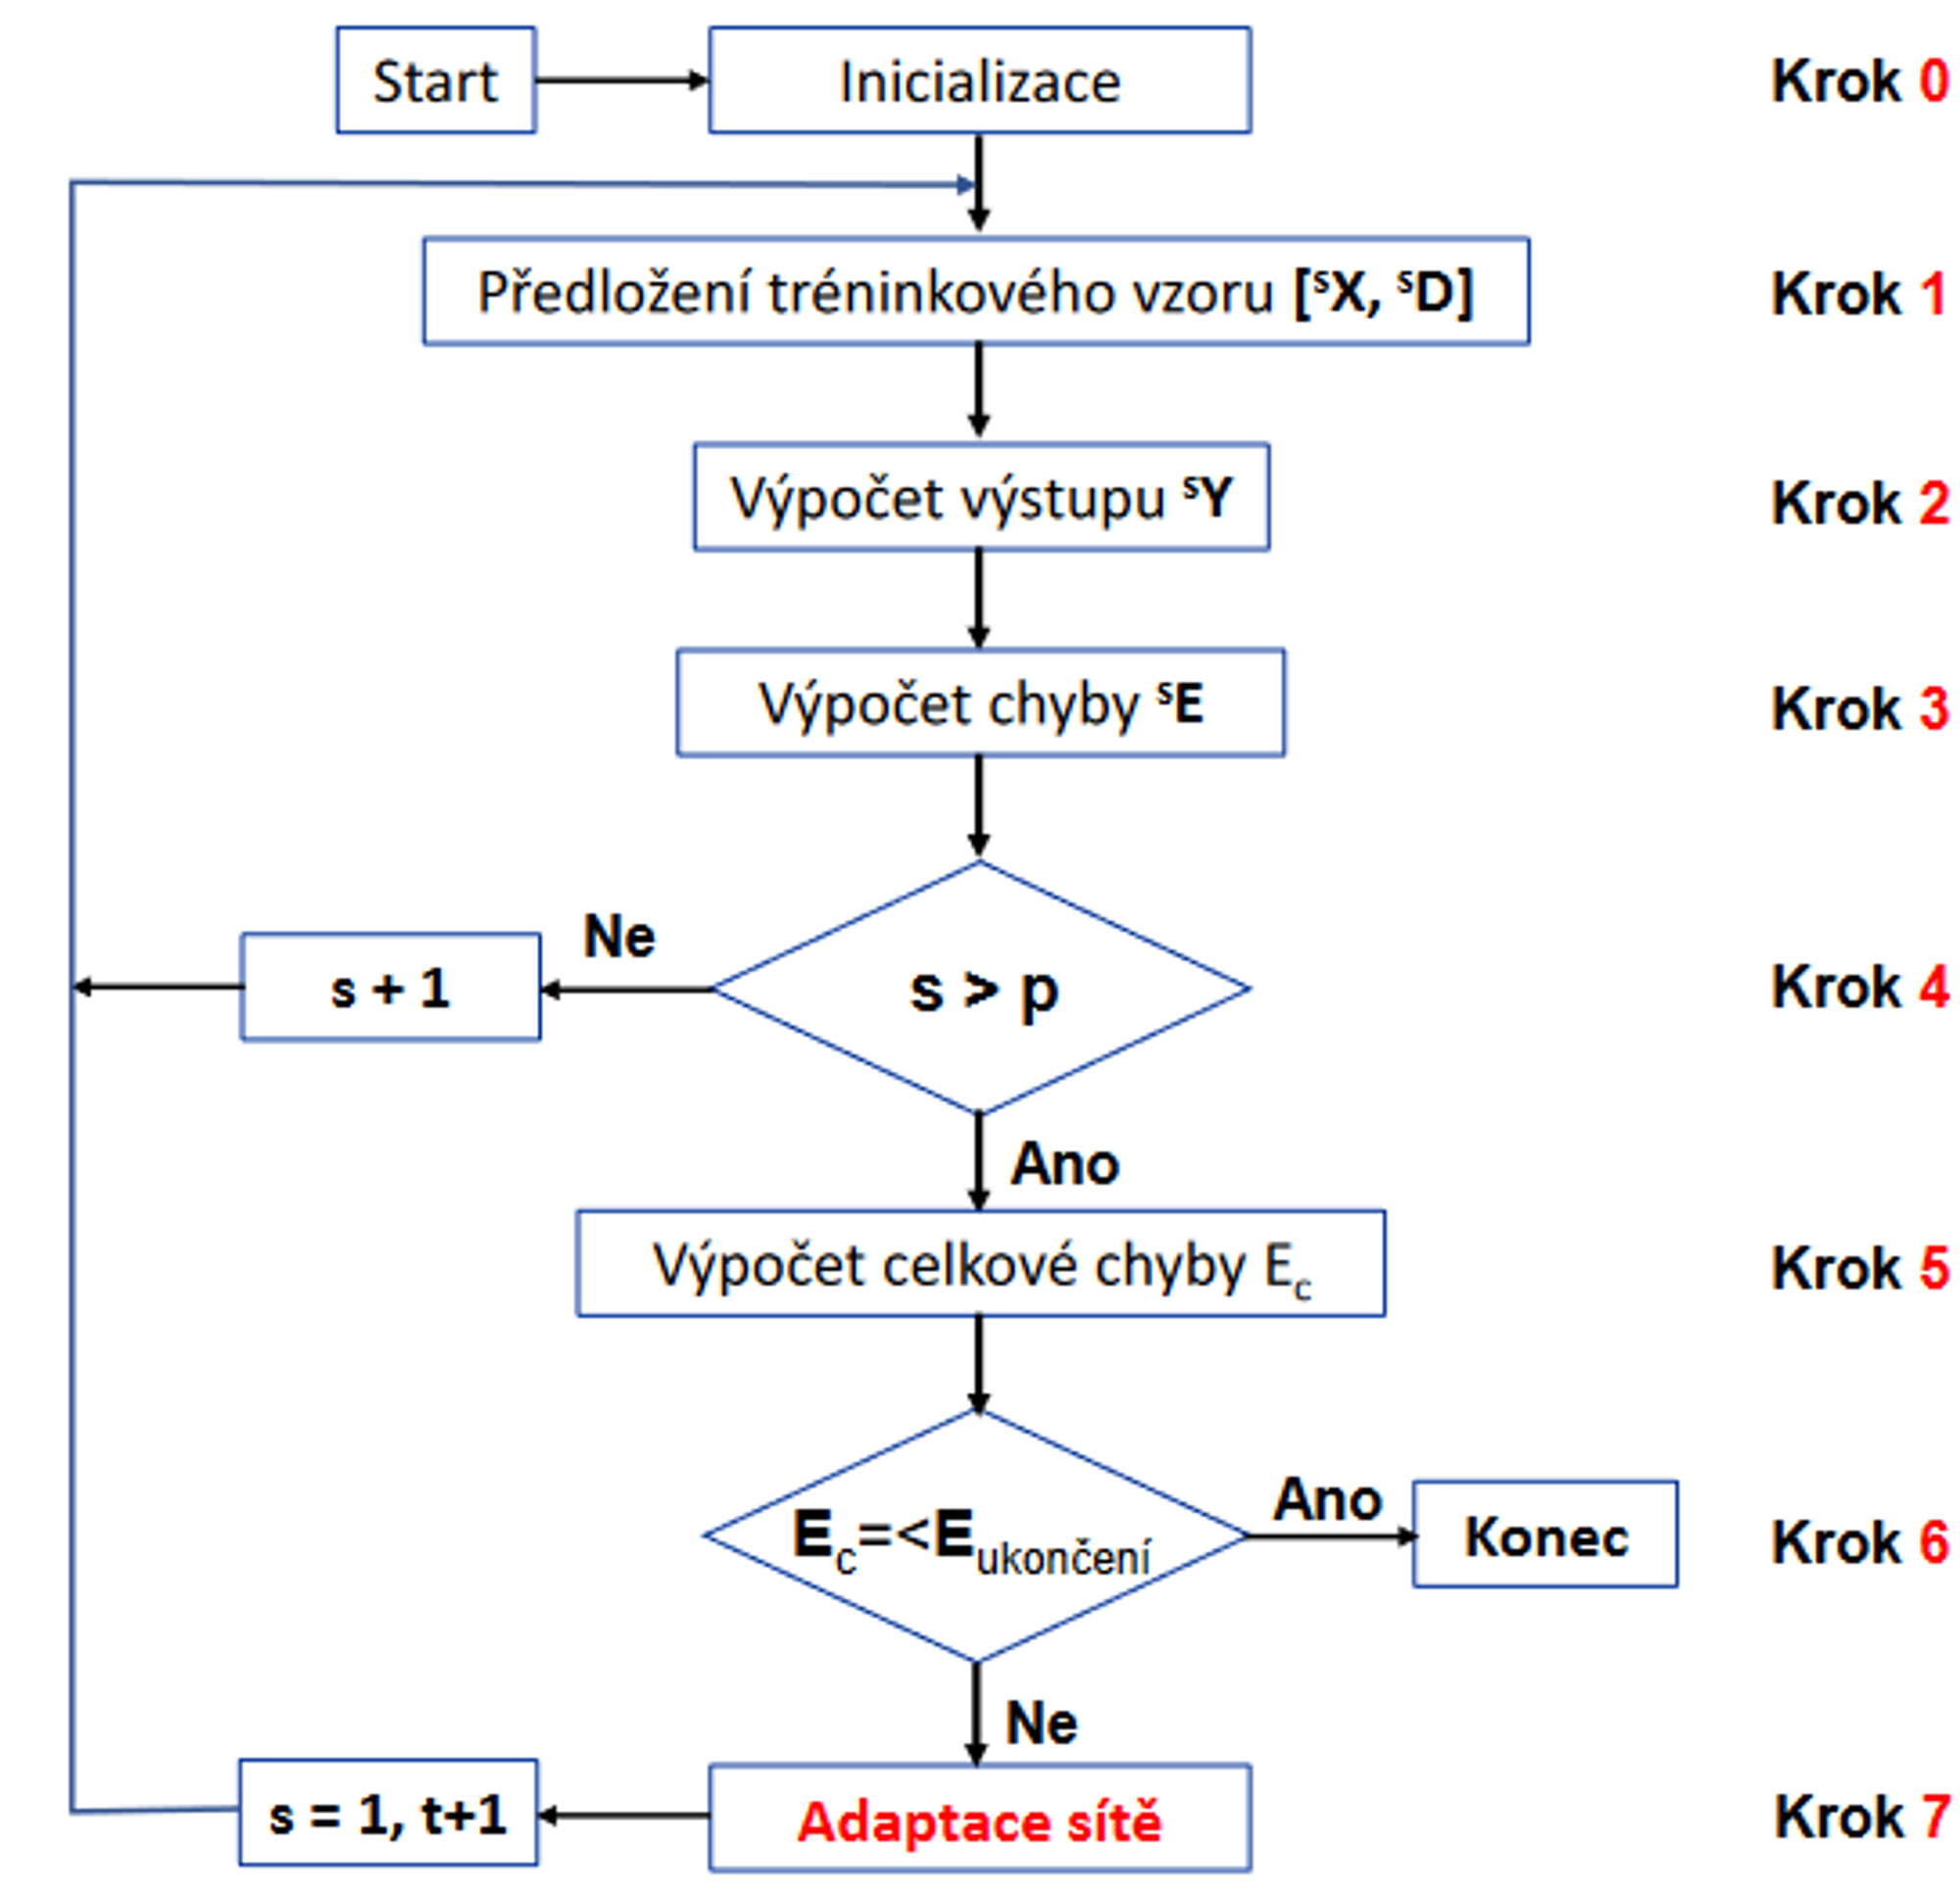
\includegraphics[scale = 0.3]{images/backPropag_uceni.png}
\end{figure}
s \dots počet tréninkových vzorů\\
p \dots celkový počet tréninkových vzorů\\
Akumulované učení - adaptace vah po předložení všech t. vzorů, nezáleží na pořadí vzorů\\
Adaptace po každém tréninkovém vzoru - záleží na pořadí vzorů, zpomaluje konvergenci

\subsection*{Kohonenova samoorganizační mapa}
soutěžní strategie učení\\
nástroj pro identifikaci neznámých vlastností a parametrů skrytých ve vstupních datech(rozmisťování zboží podle toho, jak lidi nakupují)\\
Charakteristika:
\begin{itemize}
    \item neuron - lineární, měření vzdálenosti
    \item topologie - dvouvrstvá s definovaným okolá ve 2.vrstvě
    \item učení - iterační proces, bez učitele
    \item vybavování - jednorázový proces
    \item apliakce - hodně naměřených dat
\end{itemize}
\subsubsection*{Neuron}
ve vstupní vrstvě lineární přenosová funkce\\
ve výstupní není přenosová funkce, zde se provádí výpočet vzdálenosti d
\begin{equation}
    d_j = \sum^n_{i=1} \left(x_i - w_{ij}(t)\right)^2 
\end{equation}
\subsubsection*{Topologie}
Dvouvrstvá síť s úplným propojení neuronů\\
výstupní vrstva je kompetiční\\
\begin{figure}[H]
    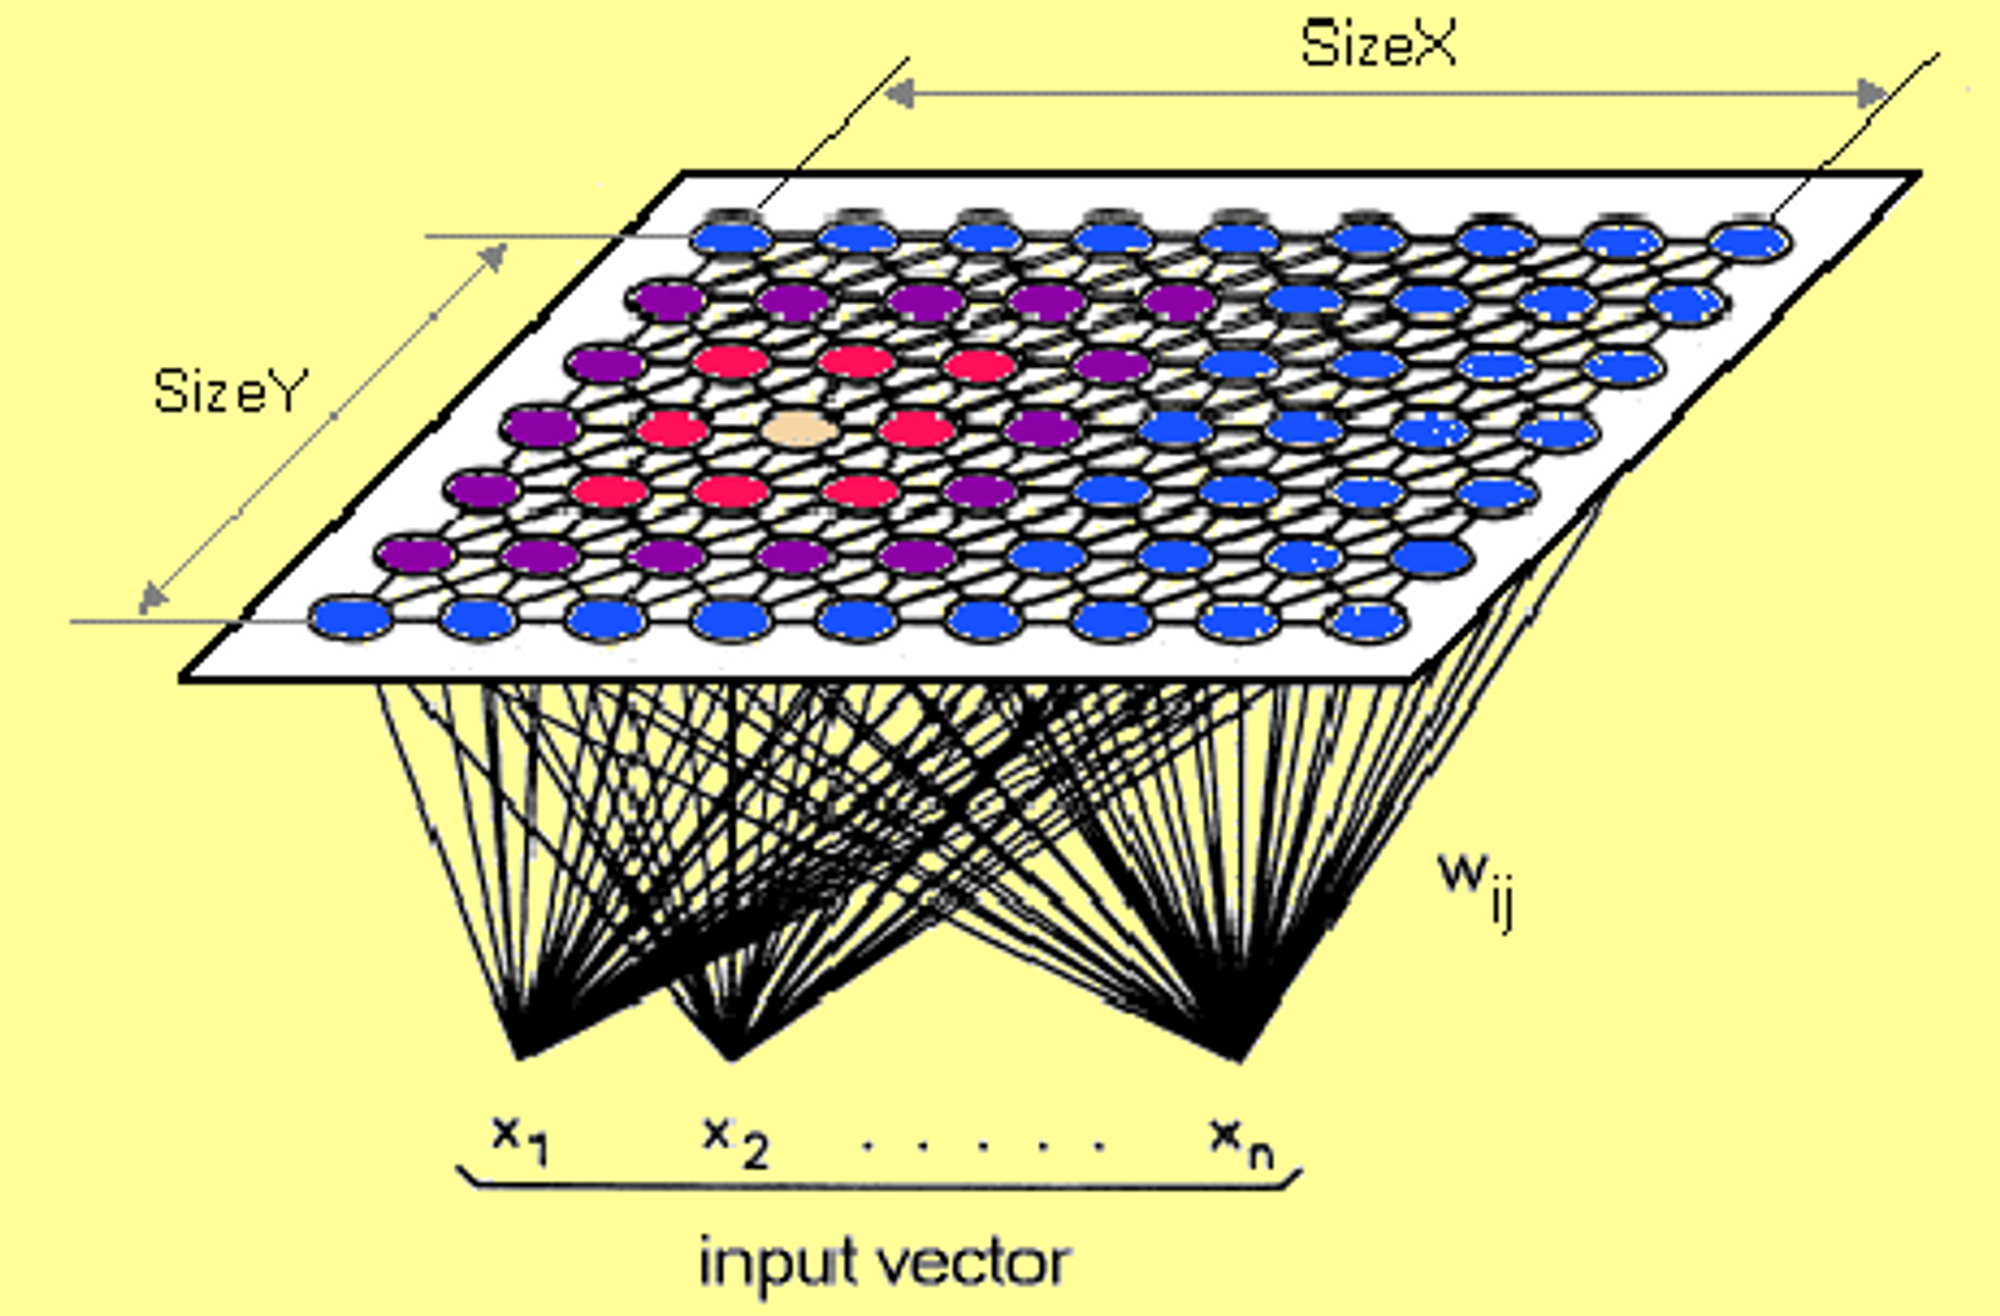
\includegraphics[scale = 0.3]{images/kohonen_topologie.png}
\end{figure}
\newpage
struktura určuje, které neurony spolu sousedí:
\begin{figure}[H]
    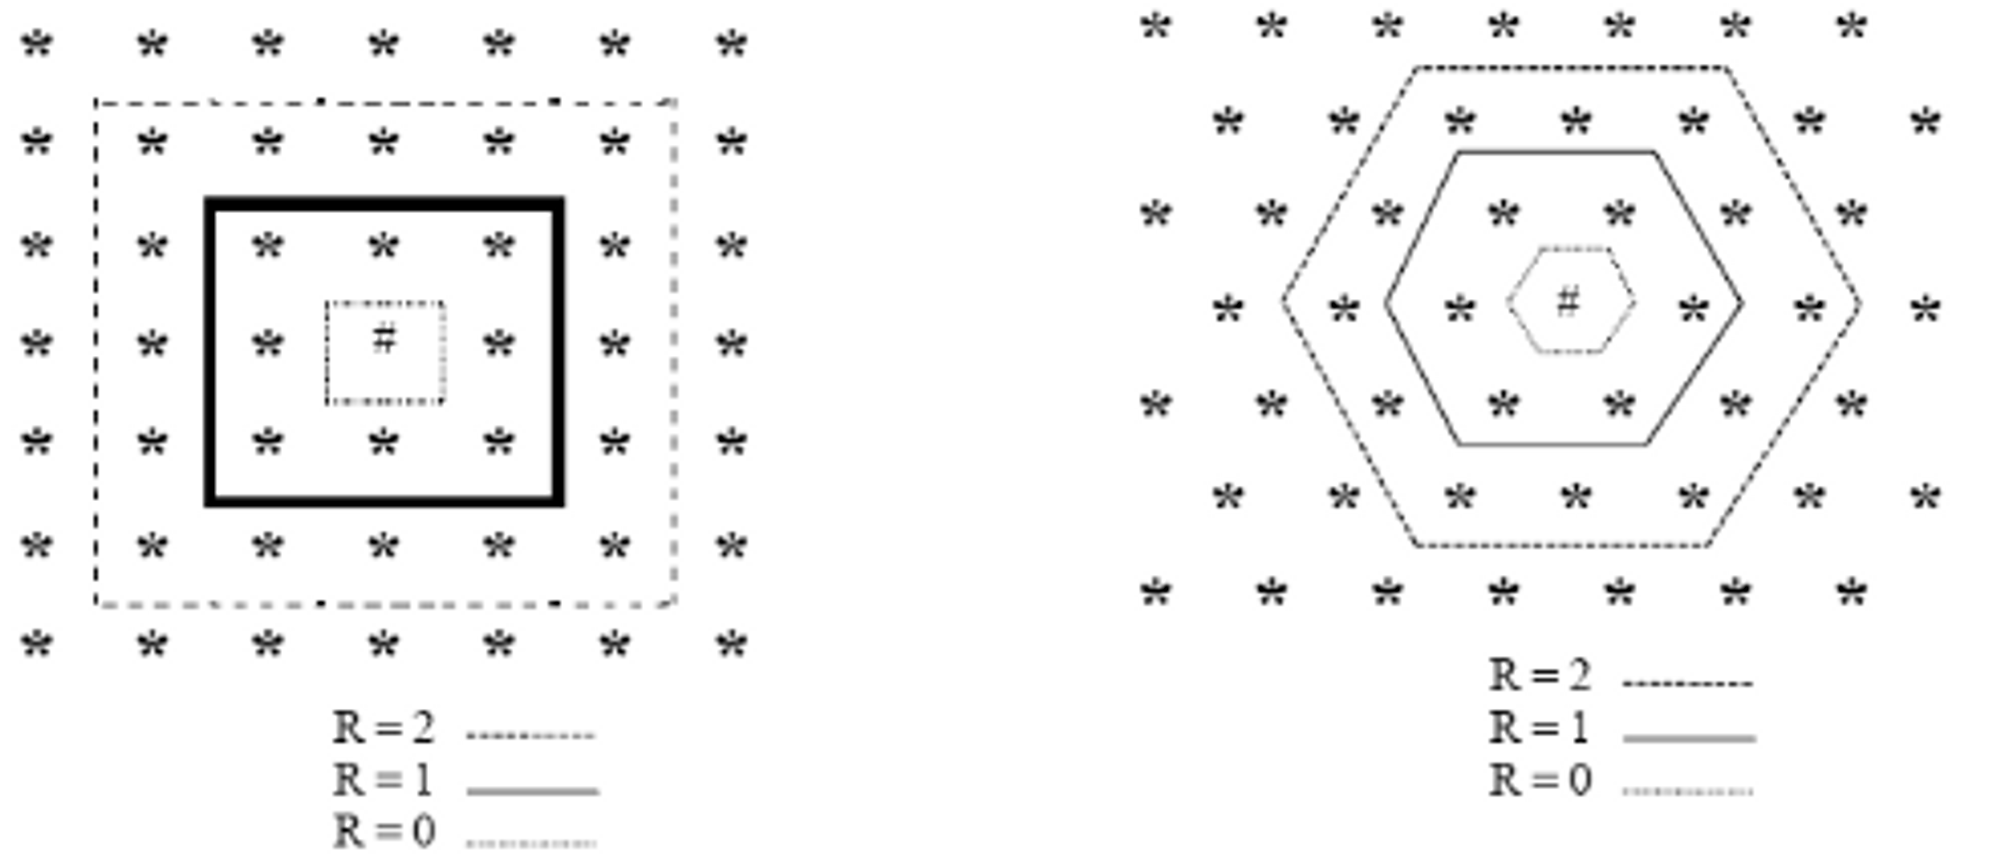
\includegraphics[scale = 0.3]{images/kohonen_struktura.png}
\end{figure}

\subsubsection*{Učení}
Váha úspěšného neuronu je zvýšena, neúspěšných je snížena\\
bez učitele\\
učení probíhá tak, že se umístí neurony kolem jednoho bodu v prostoru(grandmother cell), následně se předloží vstupní data a najde se neuron s nejmenší vzdáleností do tréninkového vzoru, který je vítěz\\
probíhá jednou pro každý tréninkový vzor\\

\subsubsection*{Vybavování}
\begin{enumerate}
    \item předložení vzoru
    \item výpočet vzdáleností
    \item nalezení vítězného neuronu
\end{enumerate}

\subsubsection*{aplikace}
\begin{itemize}
    \item zpracování řeči, obrazu
    \item hledání a detekce osob podle fotografií
    \item přepis ručně psaného textu na tištěný
    \item automatické třídění 
\end{itemize}
\newpage

\subsection*{Konvoluční neuronová síť}
Typické využití u zpracování obrazu\\
Konvoluce je matematický operátor pro spojování dvou funkcí.\\
Má konvoluční jádro, kterým prochází každý prvek obrazu/pole\\
Topologie vícevrstvá neuronová síť\\
Vstupní obraz se musí většinou zkomprimovat pomocí konvoluce a poolingu\\

\begin{figure}[H]
    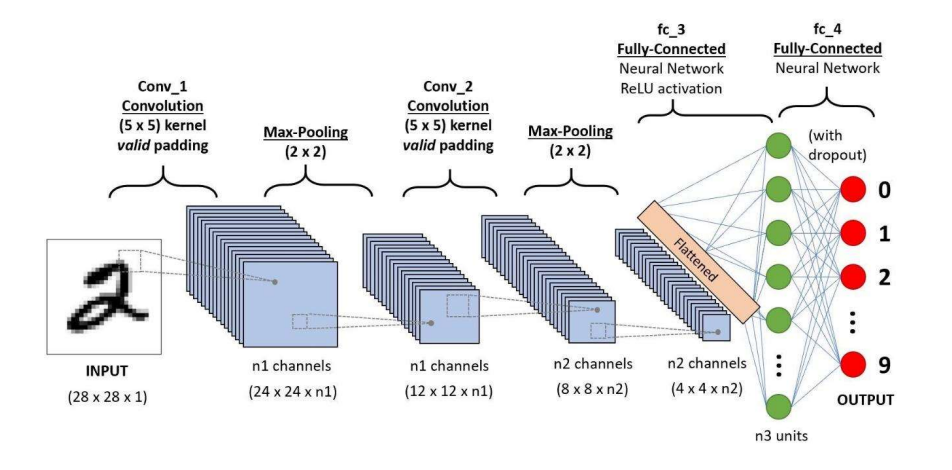
\includegraphics[scale = 1]{images/konvoluce.png}    
\end{figure}
\newpage

\section{Expertní systémy(ES) - definice, architektura, teoretické zdroje pro realizaci ES, tvorba a ladění báze znalostí, průběh konzultace}
Počítačové programy, které simulují rozhodovací činnost experta při řešení velmi složitých úloh a využívají vhodně zakódovaných speciálních znalostí převzatých od experta\\
ES jsou využívány tam, kde neexistuje dostatečné algoritmické řešení a jediným možným řešením je určitá forma usuzování.\\
Charakteristické rysy:
\begin{itemize}
    \item neurčitost v bázi znalostí
    \item neurčitost v odpovědích uživatele
    \item dialogový režim
    \item vysvětlovací činnost
    \item modularita a transparentnost báze znalostí
\end{itemize}

\subsubsection*{Role ES}
asistent - pomůcka experta na potvrzení či zpochybnění svých profesionálních názorů\\
kolega - expertní systém navrhuje řešení, konečné rozhodnutí dělá uživatel\\
expert - pracuje úplně autonomně na úkolech, které uživatel není schopen vyřešit\\
\newpage
\subsubsection*{Architektura}
Zjednodušenná verze:
\begin{figure}[H]
    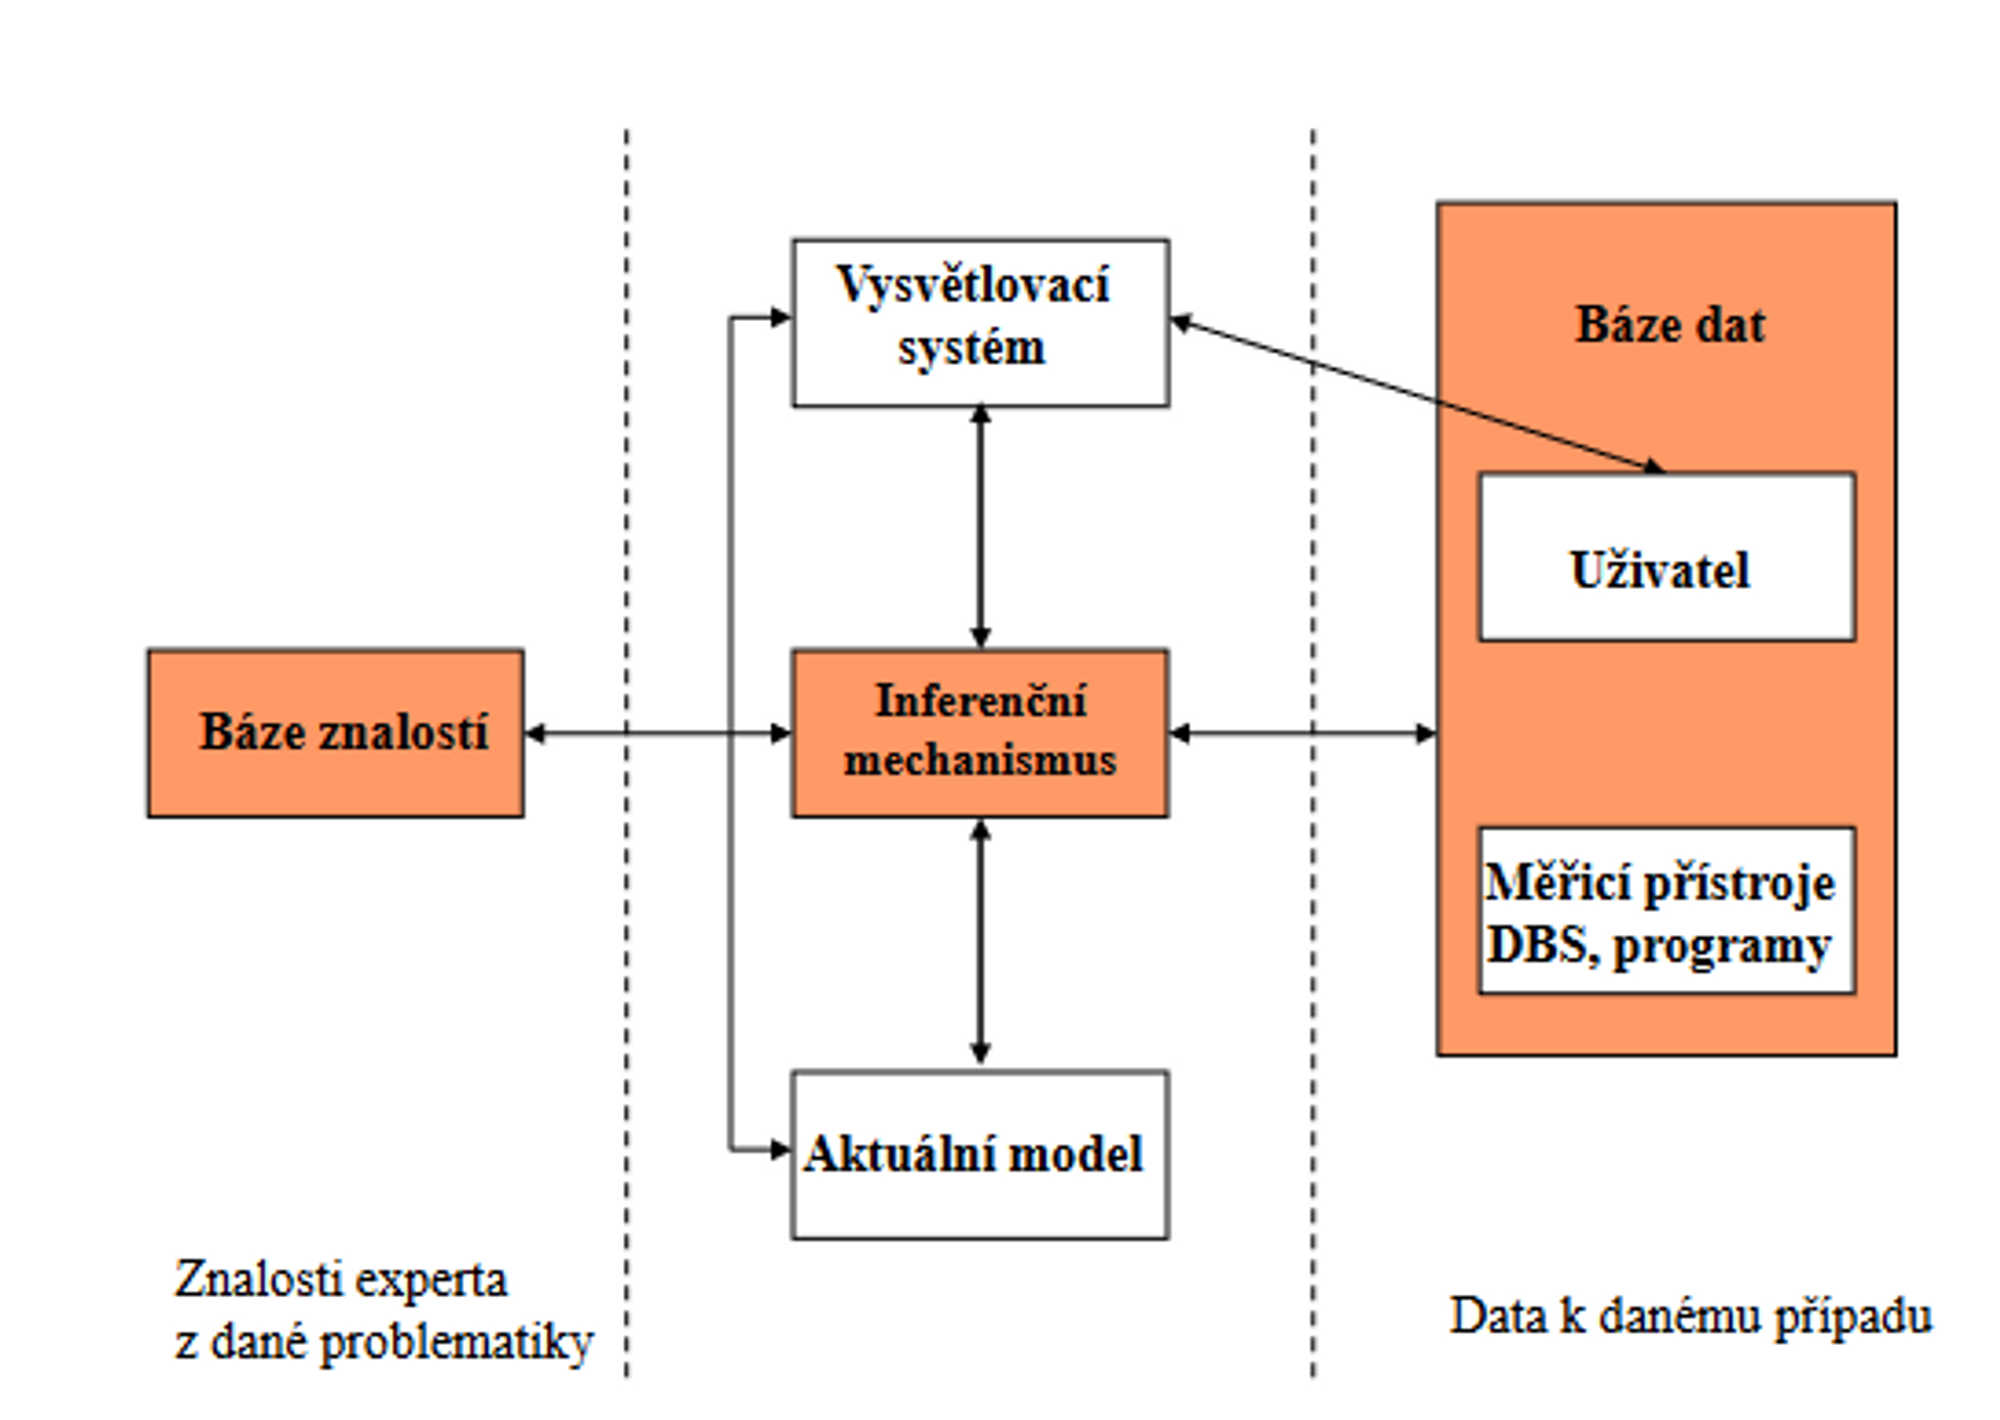
\includegraphics[scale = 0.3]{images/ES_ez.png}    
\end{figure}
Inferenční mechanismus
\begin{itemize}
    \item Zajišťuje komunikaci s uživatelem prostřednictvím uživatelského rozhraní - dialogový režim
    \item obsahuje obecné algoritmy schopné řešit problémy na základě manipulace se znalosti z báze znalostí
    \item určuje jak a v jakém pořadí aplikovat pravidla na bázi dat
    \item založen na inferenčním pravidle odvozování nových poznatků nebo na prohledávání báze znalostí
\end{itemize}
Báze znalostí - vytváří se v průběhu řešení konkrétního problému a obsahuje data k řešenému problému\\
Aktuální model - reprezentace současného stavu řešení - v průběhu konzultace vyjádřen pravděpodobností\\
vysvětlovací modul - vysvětlení položené otázky,zdůvodňuje postup při řešení problému, odlišuje ho od znalostního systému
\newpage
\subsubsection*{Typy ES}
Obecné rozdělení:
\begin{itemize}
    \item 90\% - diagnostický
    \item 9\% - generativní/plánovací
    \item 3\% - dedikovaný/smíšený
\end{itemize}
Podle obsahu báze znalostí:
\begin{itemize}
    \item prázdný
    \item naplněná
\end{itemize}

Diagnostický:
\begin{itemize}
    \item úkolem určit, která hypotéza nejlépe koresponduje s daty týkající se daného případu
    \item pracují s pevným počtem cílů, z nichž vybírají svá doporučení
\end{itemize}
Plánovací
\begin{itemize}
    \item je znám počáteční stav a cíl řešení
    \item cíl nalézt posloupnost kroků, který k cíli dovede
    \item znalost experta + data: omezené množství řešení
\end{itemize}

Smíšený - funguje na základě střdání jednotlivých přístupů podlde potřeby\\

\subsection*{Teoretické zdroje}
Reprezentace znalostí
\begin{itemize}
    \item Deklarativní - jednotlivá fakta
    \item proceduální - znalosti ve formě procesů
    \item pravidla, rozhodovací stromy
\end{itemize}
Řešení úloh a prohledávání stavového prostoru(inferenční mechanismus)
\begin{itemize}
    \item prohledávání stavového prostoru
    \item rozklad na podproblémy
    \item dedukce - odvození závěru z předpokladu
    \item abdukce - usuzování ze závěru k předpokladu
    \item indukce - postup od specifického případu k obecnému
\end{itemize}
Zpracování neurčité informace
\begin{itemize}
    \item neurčitost - nejisté znalosti, vágní pojmy, nekonzistence dat
    \item fuzzy logika
\end{itemize}

\subsection*{Tvorba a ladění báze}
\subsubsection*{Identifikace problému}
musí se jednat o problém složitý rozsahem nebo neurčitostí vztahů, pro nějž exaktní metoda řešení není\\
provede se analýza požadavků, nalezení klíčových slov a specifikace vztahů mezi nimi

\subsubsection*{Návrh koncepce}
stanovení cíle a funkce systému\\
identifikace možných zdrojů znalostí\\
ucelená představa rozkladu na dílčí úlohy\\

\subsubsection*{Volba reprezentace znalostí}
rozhodování o typu formální prezentace znalostí na základě identifikace problému\\
viz reprezentace znalostí\\

\subsubsection*{Získávání znalostí}
interview experta nebo automatizované získávání znalostí(strojové učení)\\
mohou nastat problémy - expert nepsolupracuje, výrazy srozumitelné jen lidem v oboru\\

\subsubsection*{Implementace}
proces naplňování báze znalostí\\

\subsubsection*{Ladění báze}
změna struktury grafu\\
nastavení pravděpodobnostních uzlů na základě testovacích konzultací\\

\subsection*{Průběh konzultace}
Má 4 fáze:
\begin{enumerate}
    \item Výběr dotazu - signifikantnější dotazy na začátek
    \item Výběr odpovědi - odpovědi v několika stupních, ovlivňují hypotézy
    \item přepočet báze znalostí - přepočet pravděpodobností
    \item ukončení - na přáni uživatele, nebo byly tázány všechny dotazy 
\end{enumerate}

\section{Počítačové vidění - předzpracování obrazu, segmentace obrazu, popis a klasifikace obrazu}
\begin{figure}[H]
    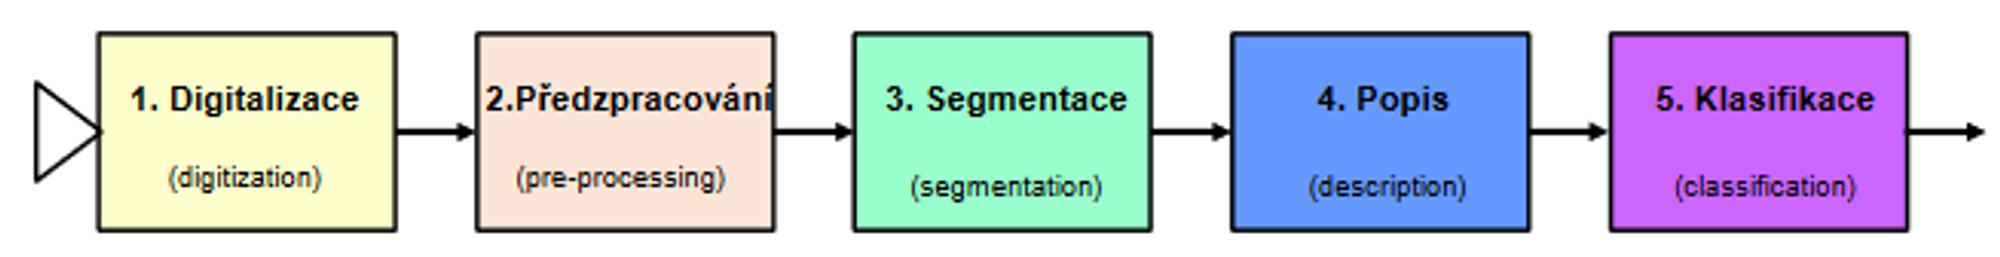
\includegraphics[scale = 0.4]{images/pc_videni.png}
\end{figure}

\subsection*{Předzpracování obrazu}
Cíle:
\begin{itemize}
    \item potlačit šum
    \item odstranit zkreslení
    \item potlačit či zvýraznit jiné rysy obrazu
\end{itemize}
Předzpracováním nezískáme žádnou novou informaci.\\
Metody předzpracování:
\begin{itemize}
    \item bodové jasové transformace
    \item geometrické transformace
    \item lokální předzpracování
    \item obnovení obrazu
\end{itemize}

\subsubsection*{Bodové jasové transformace}
Závisle na pozici:
\begin{itemize}
    \item zdroj poruch vzniklý při digitalizaci a přenosu obrazu
    \item systematické chyby lze potlačit na základěznalosti odchylky citlivosti každého bodu od ideální převodní charakteristiky:
      $f(i,j) = e(i,j)\cdot g(i,j)$\\
    Násobíme degradačním koeficientem g
\end{itemize}
\newpage
Nezávislé na pozici:
\begin{figure}[H]
    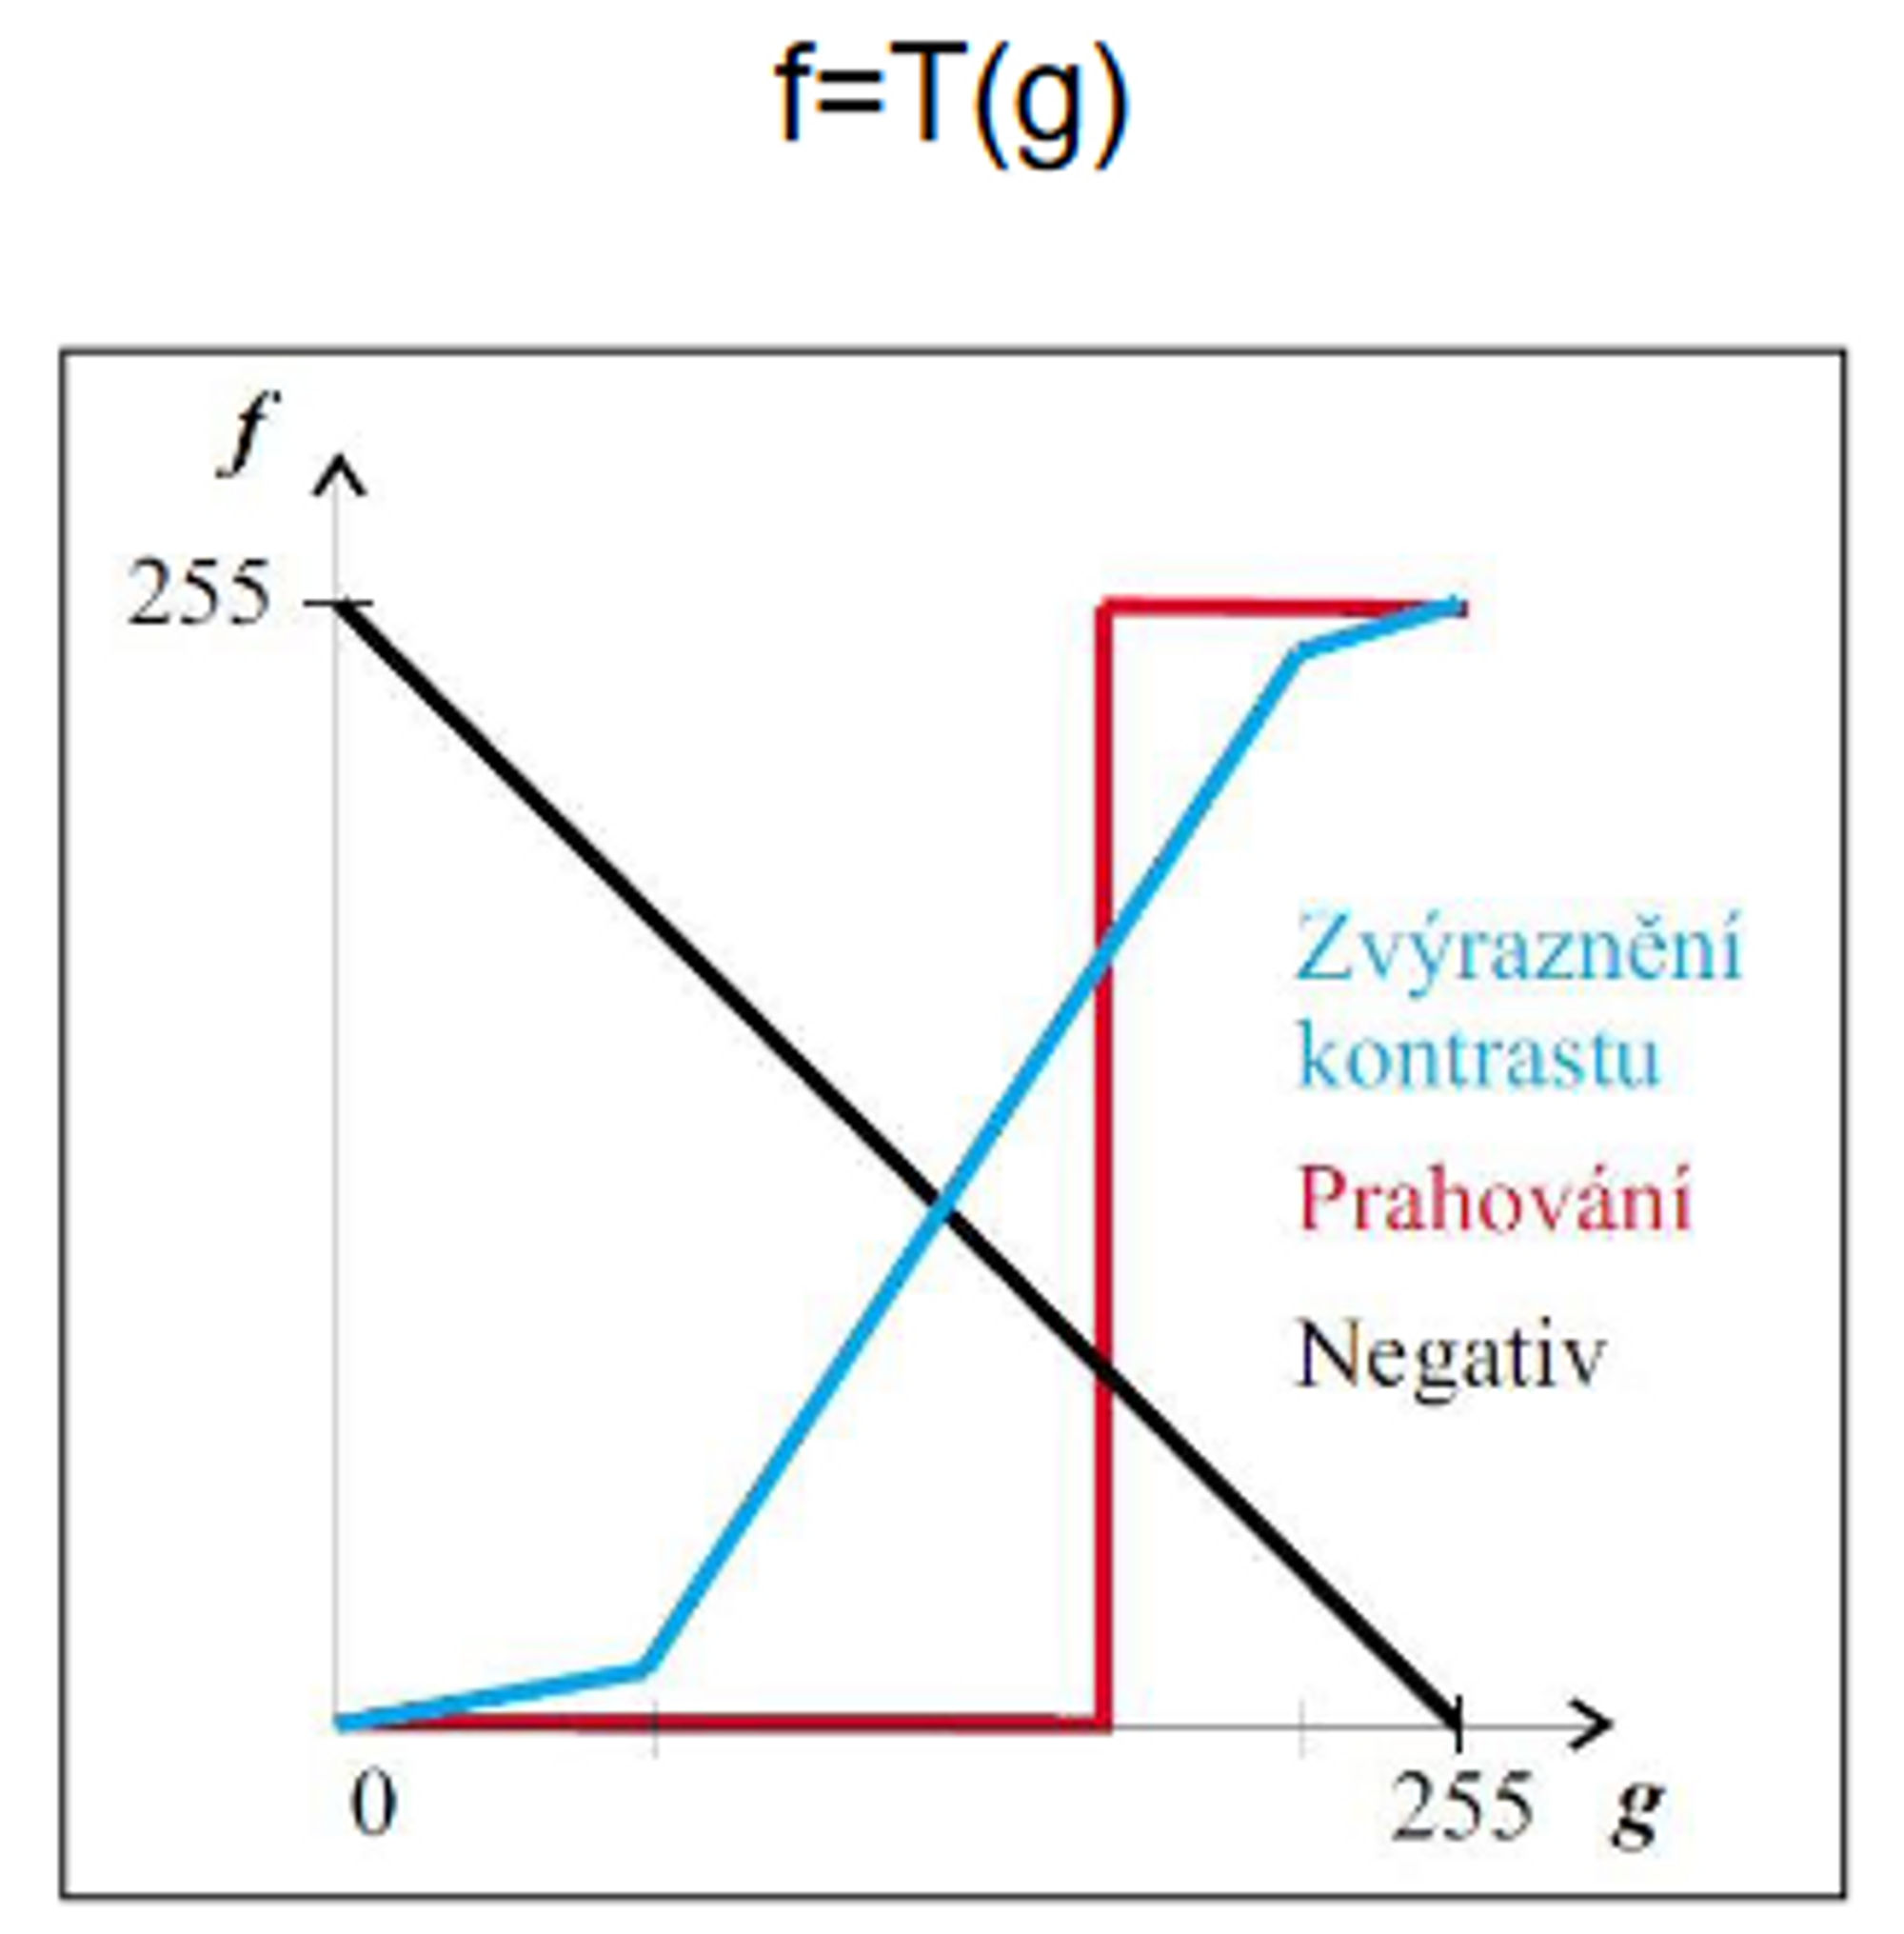
\includegraphics[scale = 0.13]{images/transf_krivka.png}
\end{figure}

\subsubsection*{Geometrické transformace}
Používají se k odstranění geometrických zkreslení.\\
Dva kroky:
\begin{itemize}
    \item plošná transformace
    \item jasová transformace
\end{itemize}
Plošná transformace:
\begin{equation}
       x' = \sum_{r =0}^m \sum_{k=0}^{m-r}a_{rk}x^ry^k, \;\;\;\; y' = \sum_{r =0}^m \sum_{k=0}^{m-r}b_{rk}x^ry^k
\end{equation}
dvojce sobě odpovídajících bod x,y a x',y'\\
Jasová transformace:
Přiřazení bodu (x,y) hodnotu jasu nejbližšího bodu v diskrétní mřížce\\
Druhá možnost je určení hodnoty poměrem vzdáleností nejbližších bodů.\\
\newpage
\subsubsection*{Lokální předzpracování}
Za účelem filtrace šumu, detekce hran, nebo ostření obrazu.\\
Filtrace:
\begin{itemize}
    \item průměrování
    \item konvoluční maska
    \item metoda mediánem
\end{itemize}
\begin{figure}[H]
    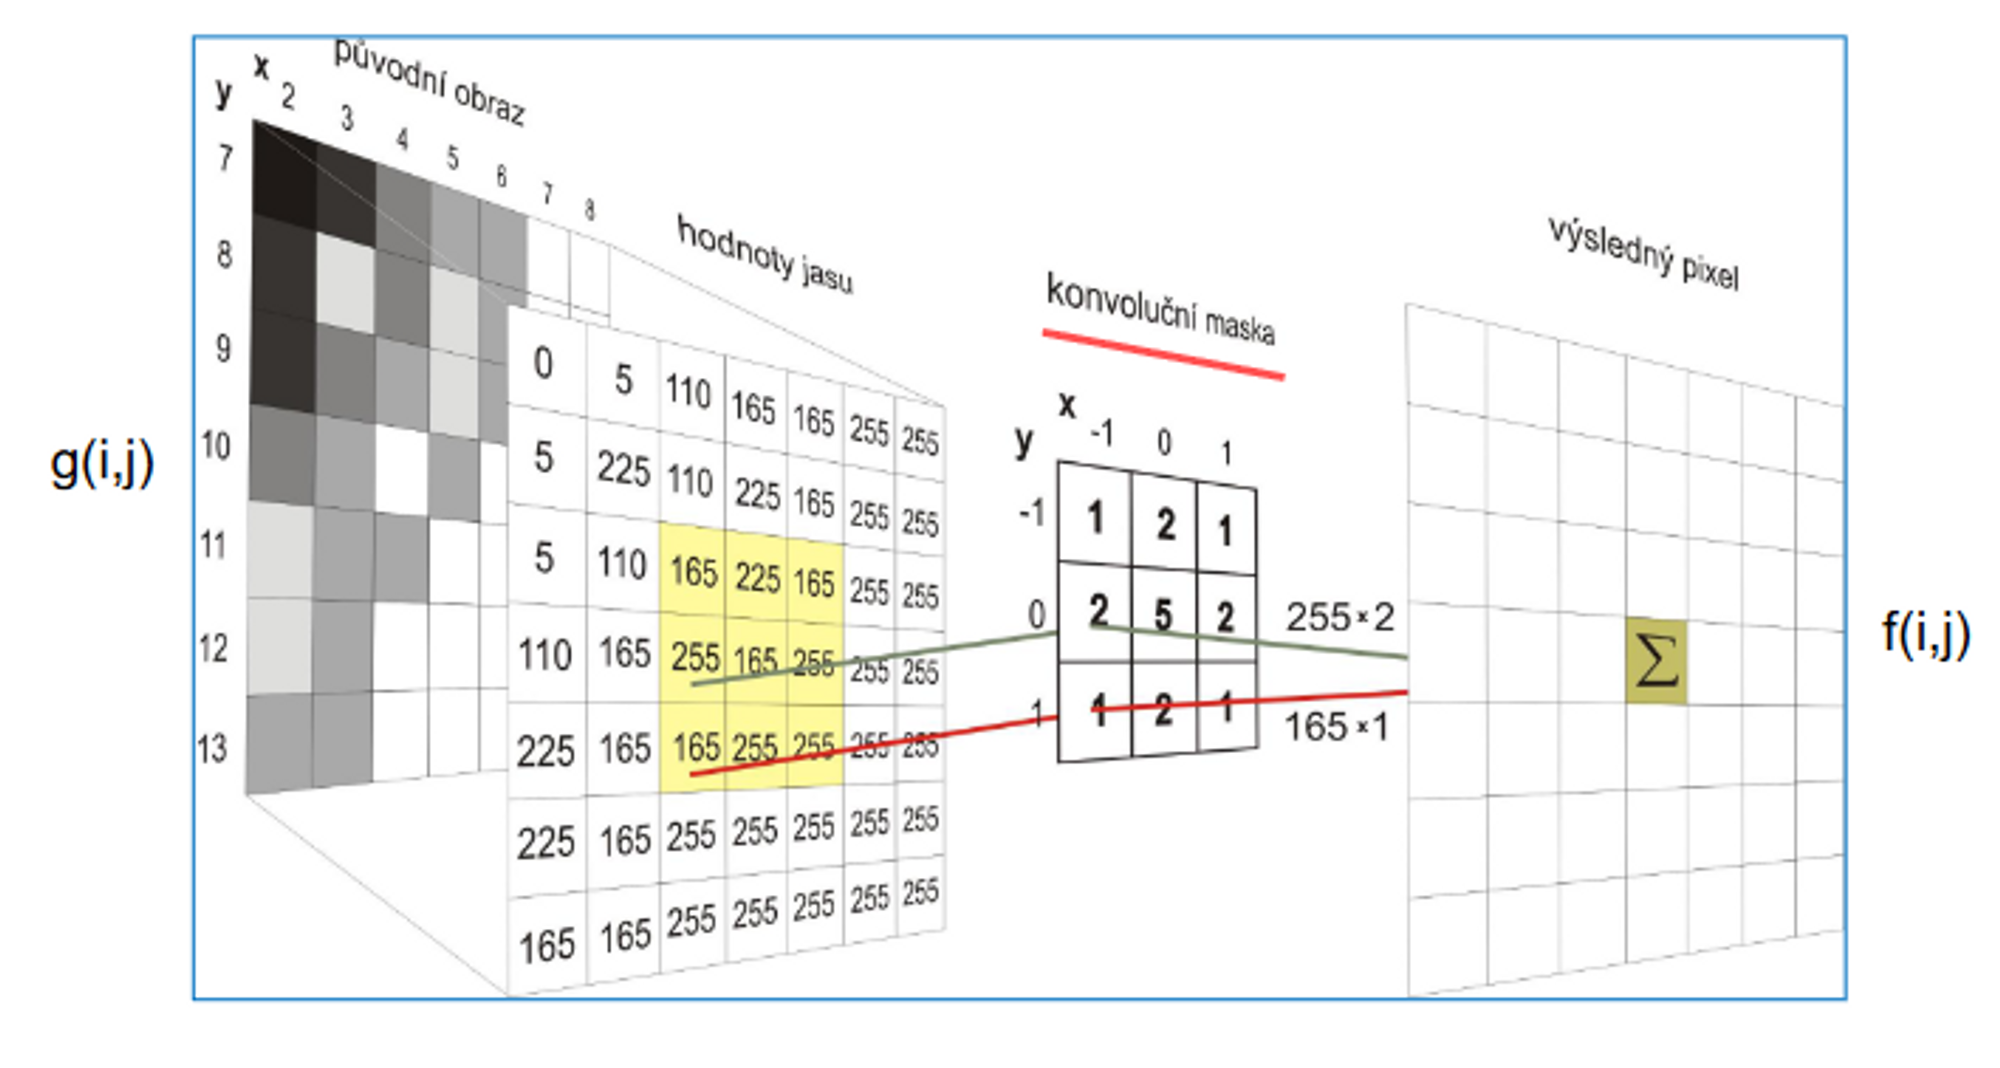
\includegraphics[scale = 0.25]{images/konvoluce_maska.png}
\end{figure}

Detekce hran:
\begin{itemize}
    \item pomocí derivačních filtrů - 1. a 2. derivace
    \item gradientní operátory
    \item laplaceovy operátory
\end{itemize}
\begin{figure}[H]
    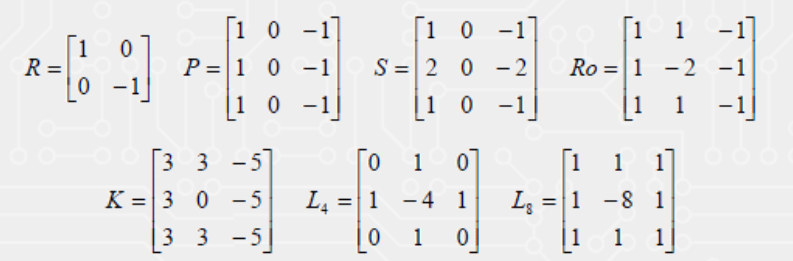
\includegraphics[scale = 0.7]{images/hrany.png}
\end{figure}
Robertsův, Prewittové, Sobelův, Robinsonův\\
Kirschův, Laplaceuv(čtyřokolí, osmiokolí)\\

\subsubsection*{Obnovení obrazu}
rozostření objektivu, rozmazání pohybujícícho se objektu\\

\subsection*{Segmentace}
Snaha rozčlenit obraz do oblastí, které mají úzkou souvislost s předměty či oblastmi reálného světa zachyceného na obrazu.\\
výsledek je soubor vzájemně nepřekrývajících se oblastí.\\
dělí se na:
\begin{itemize}
    \item kompletní - oblasti jednoznačně korespondují s objekty vstupního brazu
    \item částečná - oblasti nemusí přío korespondovat s objekty
\end{itemize}
Cíl připravit data pro popis a redukovat objem dat.\\
Metody:
\begin{itemize}
    \item prahování
    \item detekce hran
    \item segmentace narůstání oblastí
    \begin{itemize}
        \item spojování oblastí
        \item štěpení oblastí
        \item štěpení a spojování oblastí
    \end{itemize}
    \item srovnání se vzorem
\end{itemize}
\begin{figure}[H]
    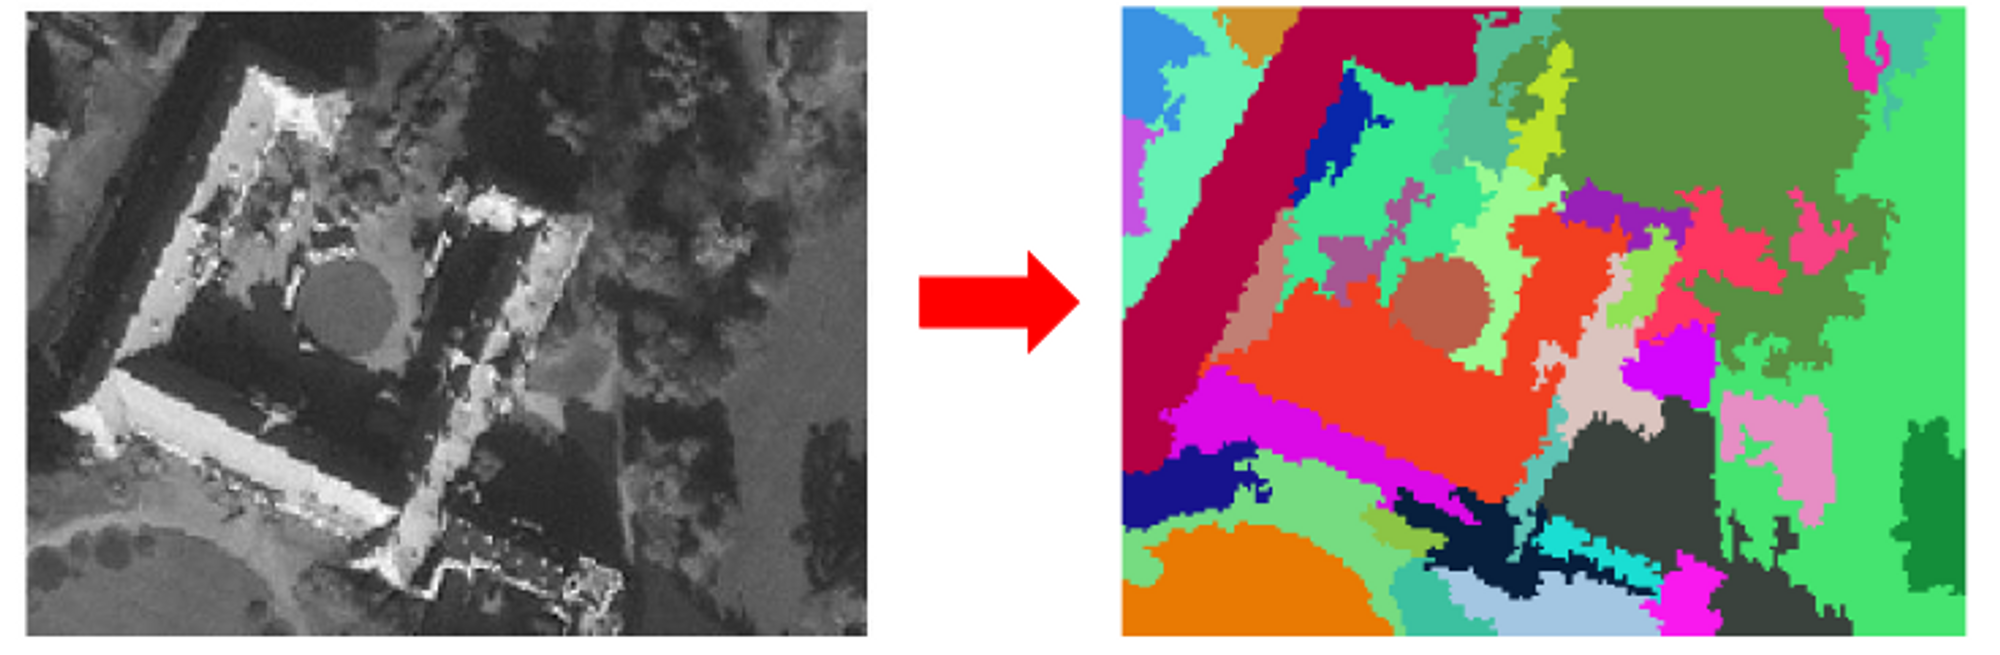
\includegraphics[scale = 0.3]{images/segmentace.png}
\end{figure}

\subsubsection*{Detekce hran}
relaxace hran - vytváření souvislých hranic\\
\newpage
\subsubsection*{Segmentace narůstání oblastí}
Spojování oblastí:
\begin{itemize}
    \item počáteční rozdělení obrazu do velkého množství malých oblastí
    \item defnice kritéria spojování
    \item spojování sousedních oblastí na základě kritéria
\end{itemize}
Štěpení oblastí:
\begin{itemize}
    \item opak spojování
    \item postupné rozkládání obrazu na menší části
\end{itemize}
Štěúení a spojování oblastí:
\begin{itemize}
    \item pyramidální reprezentace obrazu
    \item je-li oblast v dané úrovni pyramidy nehomogenní, je rozštěpena na 4 podoblasti
    \item jsou-li oblasti navzájem homogenní a lze je ve vyšší úrovni spojit do jedné, jsou spojeny
\end{itemize}

\subsection*{Popis}
Snaha určit příznaky obrazu - tvary\\
Popis musí být být invariantní proti - posunutí, měřítku, natočení, jasu a šumu.\\
\subsubsection*{Skalární popisy}
velikost, výška, šířka, výstřednost(poměr délek nejdelších na sebe kolmých tětiv), podlouhlost(poměr mezi délkou a šířkou pravoúhelníku opisující oblast)\\
\newpage
\subsubsection*{Chani codes}
řetězení, řetězové kódy\\
\begin{figure}[H]
    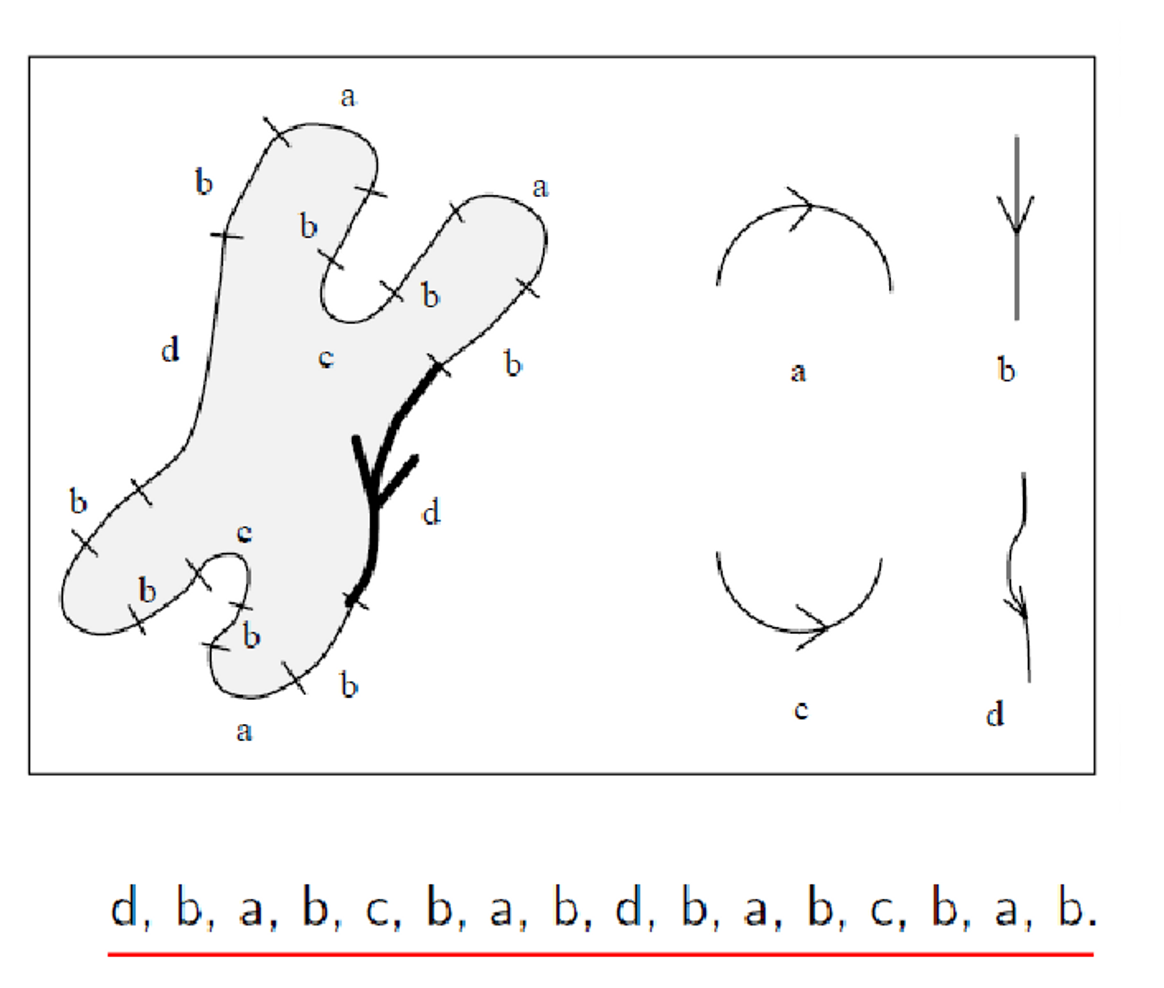
\includegraphics[scale = 0.3]{images/chain_codes.png}
\end{figure}
\subsubsection*{geometrický popis}
přímost hranice - poměr mezi celkovým počtem bodů hranice a počtem bodů, ve kterých hranice mění směr\\
\begin{figure}[H]
    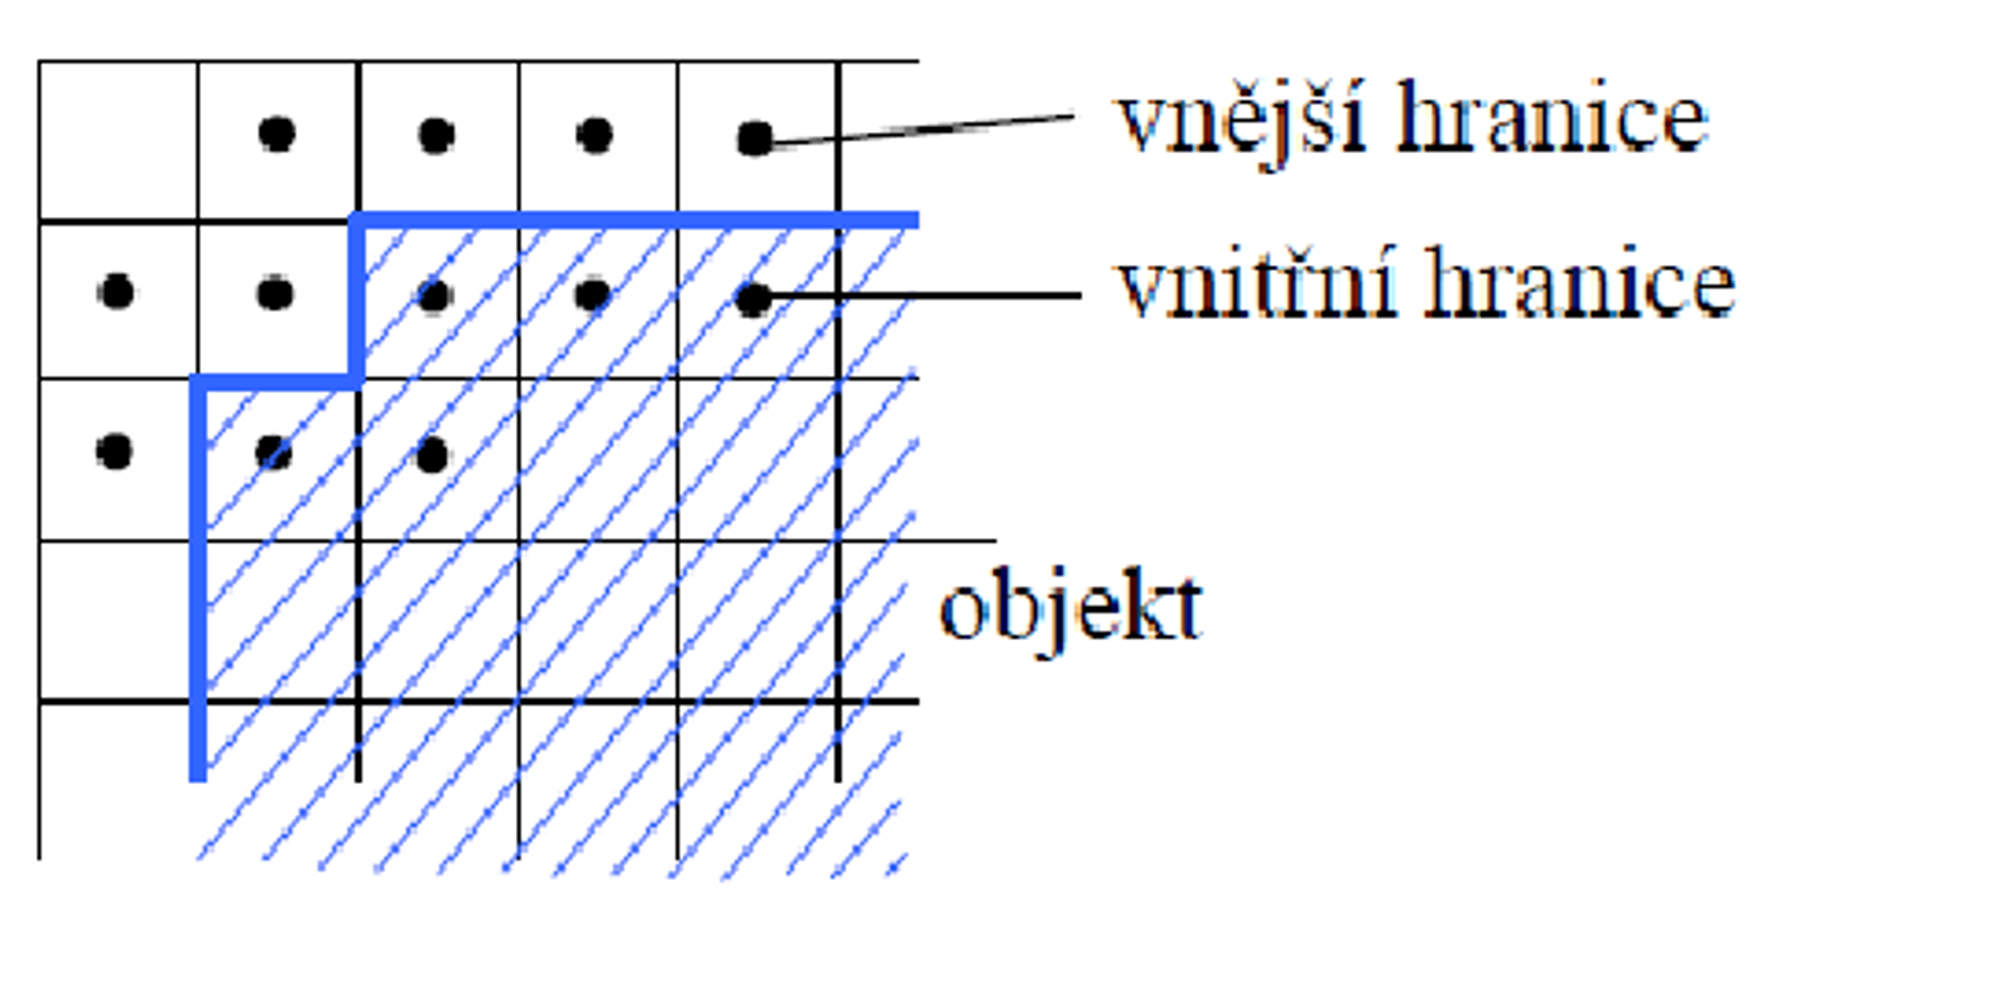
\includegraphics[scale = 0.2]{images/geometricky_popis.png}
\end{figure}
\newpage
\subsection*{Klasifikace}
rozpoznávání předmětů spočívá v jejich zařazování do tříd - klasifikátor\\
Metody rozpoznání:
\begin{itemize}
    \item příznakové - zaměřují se na měřitelné veličiny objektu
    \item syntaktické - identifikace elementů objektu a analýza vztahů mezi nimi
    \item hybridní
\end{itemize}
(jsou i další, toto jsou ty hlavní)\\
\subsubsection*{Učení}
\begin{enumerate}
    \item volba formálního popisu
    \item návrh rozhodovacího pravidla klasifikátoru
    \item způsob učení klasifikátoru - s učitelem, bez učitele
\end{enumerate}
\subsubsection*{Příznakově popsané předměty}
obraz je sloupcový vektor, jehož souřadnice tvoří vektory\\
jednotlivým třídám odpovídají shluky obrazů, které lze oddělit vhodnou křivkou pomocí diskriminačních funkcí

\begin{figure}[H]
    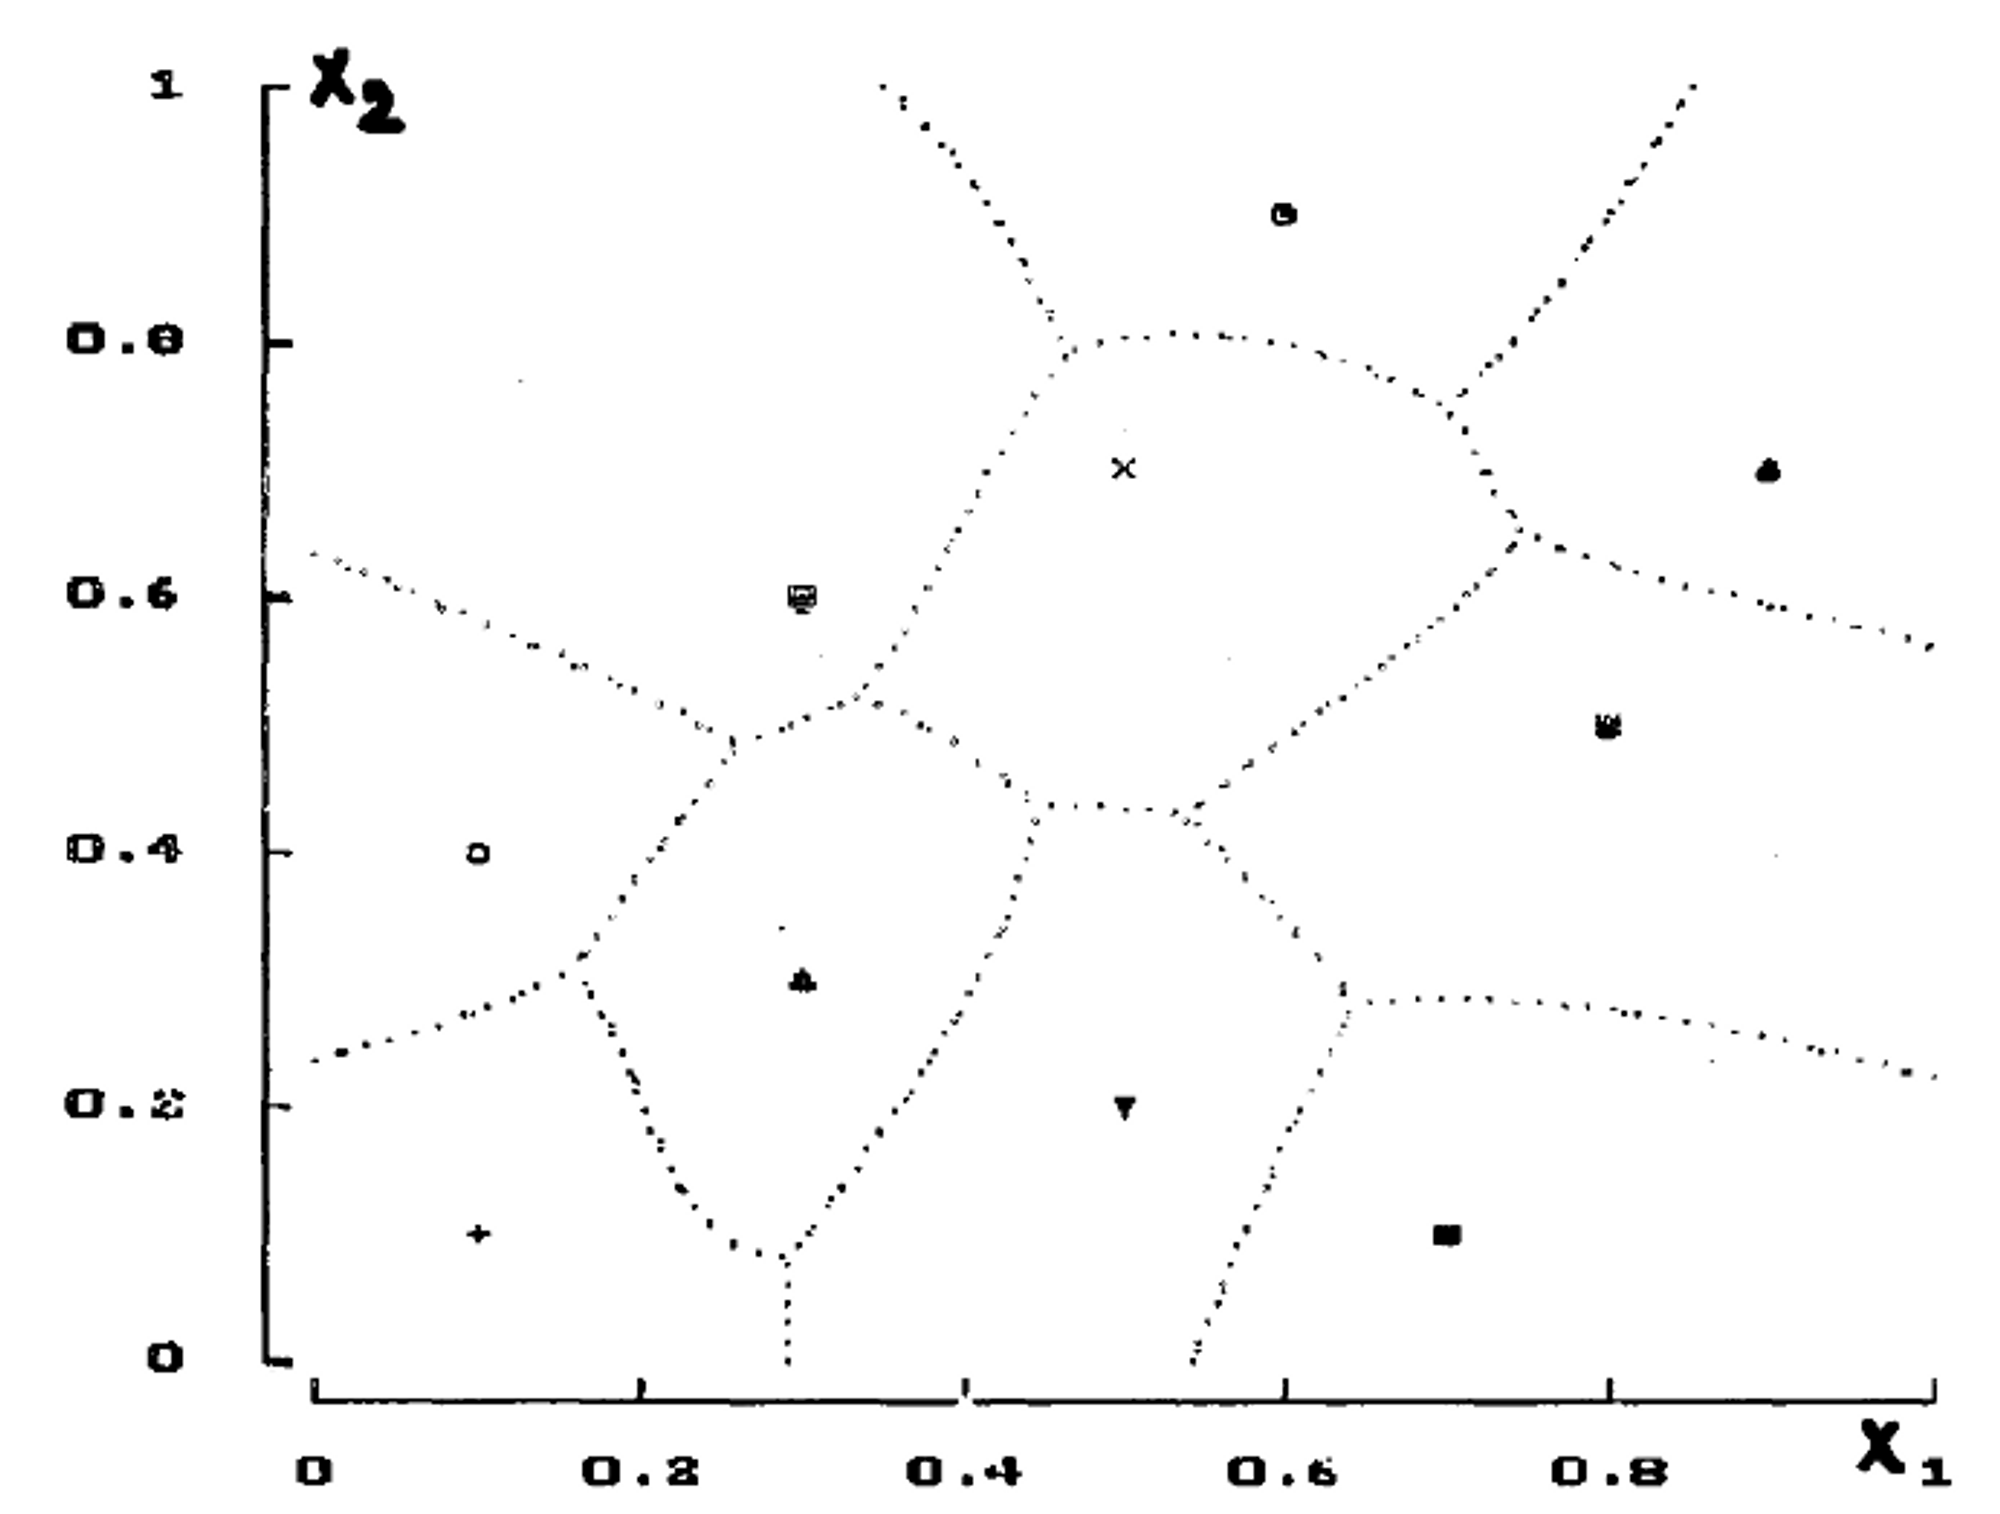
\includegraphics[scale = 0.2]{images/priznakove.png}
\end{figure}
\newpage
\subsubsection*{Syntakticky popsané předměty}

Identifikace elementů objektu a analýza mezi nimi\\
využívá primitiva, což jsou základní vlastnosti objektu, který popisují\\
primitiva se dávají do souvislostí
\begin{figure}[H]
    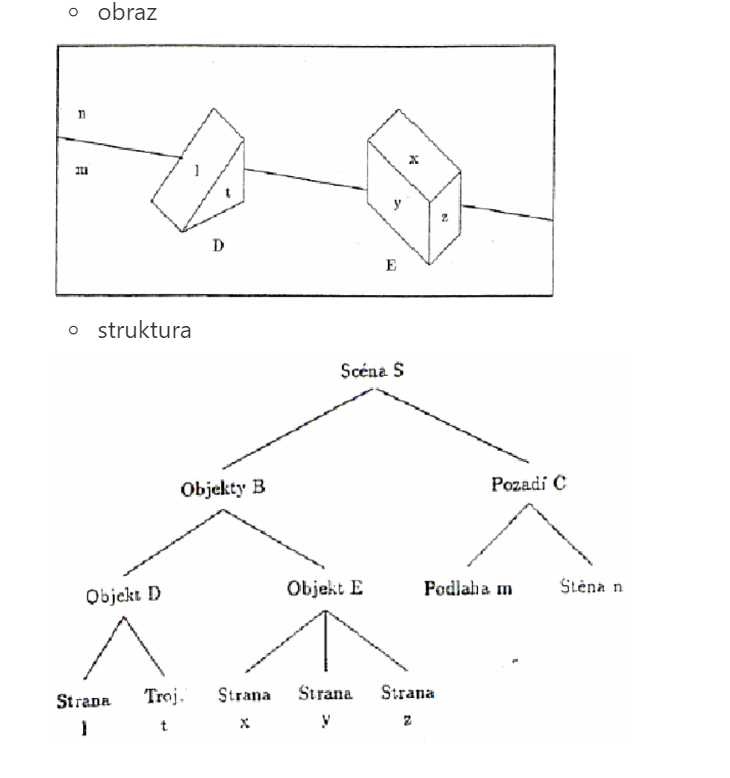
\includegraphics[scale = 0.7]{images/syntakticke.png}
\end{figure}
